\documentclass[oneside]{fduthesis}

\fdusetup{
  style = {
    font = lm,
    % 西文字体(包括数学字体)
    % 允许选项:
    %   font = garamond|libertinus|lm|palatino|times
    %
    % 注意:
    %   1. LaTeX 默认风格是 lm
    %   2. Satoshi 的讲义风格是 palatino
    %
    cjk-font = windows,
    % 中文字体
    % 允许选项:
    %   cjk-font = adobe|fandol|founder|mac|sinotype|sourcehan|windows
    %
    % 注意:
    %   1. 中文字体设置高度依赖于系统。各系统建议方案:
    %        windows:cjk-font = windows
    %        mac:    cjk-font = mac
    %        linux:  cjk-font = fandol(默认值)
    %   2. 除 fandol 和 sourcehan 外,其余字体均为商用字体,请注意版权问题
    %   3. 但 fandol 字体缺字比较严重,而 sourcehan 没有配备楷体和仿宋体
    %   4. 某些字体会有 Font "xxx" does not contain requested Script "CJK" 的警告,可以忽略
    %
    font-size    = -4,
    bib-backend  = bibtex,
    bib-resource = {main.bib}
  },
  info = {
      title            = {数值Bootstrap及其在凝聚态物理中的应用},
      % title            = {如果标题很长,可以用英文逗号分成两行},
      author           = {吴晋渊},
      department       = {物理学系},
      major            = {物理学},
      supervisor       = {戚扬},
      supervisor-title = {研究员},
      affiliation      = {物理学系},
      student-id       = {18307110155},
      keywords         = {Bootstrap, Hubbard模型, 非简谐振子},
      keywords*        = {Bootstrap, Hubbard model, nonlinear oscillator},
      % 中英文关键字均使用英文逗号分隔
  }
}

\unimathsetup{math-style=TeX}

% 需要的宏包可以自行调用
\usepackage{booktabs}
\usepackage{amsmath}
\usepackage{mathtools}
\usepackage{siunitx}
\usepackage{physics}
\usepackage{tikz}
\usepackage{cancel}
\usepackage{color}
\usepackage{array}
\usepackage{verbatim}
\usepackage{multirow}
\usepackage{tabularx}
\usepackage{extarrows}
\usepackage{listings}
\usepackage{subcaption}
\usepackage[linkcolor=black,menucolor=black]{hyperref}
\usepackage{prettyref}

\usetikzlibrary{fadings}
\usetikzlibrary{patterns}
\usetikzlibrary{shadows.blur}
\usetikzlibrary{shapes}

\newrefformat{chap}{第\ref{#1}章}
\newrefformat{sec}{第\ref{#1}节}
\newrefformat{note}{注\ref{#1}}
\newrefformat{fig}{图\ref{#1}}
\newrefformat{alg}{算法\ref{#1}}
\newrefformat{tbl}{表\ref{#1}}

\newcommand{\hilbertH}{\symcal{H}}
\newcommand{\ee}{\symrm{e}}
\newcommand{\ii}{\symrm{i}}

\newcommand{\concept}[1]{\textbf{#1}}

% Disable unsupported commands in bookmark titles 
\pdfstringdefDisableCommands{%
  \def\\{}%
  \def\texttt#1{<#1>}%
  \def\mathbb#1{#1}%
}
\pdfstringdefDisableCommands{\def\eqref#1{(\ref{#1})}}

\makeatletter
\pdfstringdefDisableCommands{\let\HyPsd@CatcodeWarning\@gobble}
\makeatother

% 图片路径
% \graphicspath{{images/}}

% 目录深度,只保留到 \section
\setcounter{tocdepth}{2}

\begin{document}

\renewcommand{\Re}{\mathrm{Re}}
\renewcommand{\Im}{\mathrm{Im}}
\newcommand{\pair}[1]{\langle #1 \rangle}

% 前置部分包含目录、中英文摘要以及符号表等
\frontmatter

% 目录
\tableofcontents
% 插图目录
%\listoffigures
% 表格目录
% \listoftables

\begin{abstract}
    数值bootstrap方法是一种新兴的数值方法,是共形bootstrap方法在一般的哈密顿量上的推广,通过物理量期望值之间的约束关系和正定性条件计算体系能量下界和其它物理量的近似值。
    本文回顾了数值bootstrap方法的形式理论和已经报道的应用,介绍了它相比已有的非微扰数值方法的优势,复现了\parencite{han_matrix}中非简谐振子的非线性SDP(半正定规划,semidefinite programming)数值bootstrap并完成了其线性SDP,并与定态薛定谔方程比较,验证了其正确性,并发现了高精度计算时的收敛性问题;复现了\parencite{han_manybody}中一维和二维Hubbard模型的线性SDP数值bootstrap,观察了其精度和Hubbard $U$参数和电子填充数目的关系,并定性分析了其原因;展望了数值bootstrap方法未来可能的发展和在其它模型上的广阔前景。
\end{abstract}

\begin{abstract*}
    As a generalization of conformal bootstrap to generic Hamiltonians, numerical bootstrap is an emerging 
    numerical method which calculates a lower bound of the energy and approximations of observables
    from constraints between quantum operators and the positivity condition.
    This thesis reviews its formalism and reported applications and its advantages compared to existing 
    non-perturbative approaches. The nonlinear SDP (semidefinite programming) numerical bootstrap of the anharmonic oscillator in 
    \parencite{han_matrix} is reproduced, and a linear SDP simulation of the anharmonic oscillator is 
    also performed, with the convergence problem with a large operator space discovered, both of which 
    are benchmarked with the stationary Schr\"{o}dinger equation. The linear SDP numerical bootstrap in 
    \parencite{han_manybody} is also produced, both for 1D and 2D Hubbard model. The correlation between 
    the precision and the Hubbard local repulsion parameter $U$ and electron filling is discussed and 
    qualitatively analyzed. The prospective developments of numerical bootstrap and its possible applications
    on other models are also discussed.
\end{abstract*}

% 主体部分是论文的核心
\mainmatter

\ctexset{chapter/pagestyle=fancy}

% 建议采用多文件编译的方式
% 比较好的做法是把每一章放进一个单独的 tex 文件里,并在这里用 \include 导入,例如
%   \include{chapter1}
%   \include{chapter2}
%   \include{chapter3}

\chapter{绪论}

\section{引言}

凝聚态物理中的传统量子多体方法从电子在周期性势场中产生的能带结构出发,通过费曼图微扰地处理库仑相互作用;大体上说,这种范式对应于朗道费米液体理论及其修正\cite{mahan2013many}。
在强关联体系中,费米液体图像失效,在量子多体理论中体现为有相互作用格林函数和无相互作用格林函数无法建立绝热演化的关系,LW泛函出现多值性等现象\cite{Gunnarsson_2017}。
已有多种数值方法可用于不借助微扰论求解强关联系统。对自旋模型,可使用世界线蒙特卡洛、随机级数展开,对电子模型,可使用行列式蒙特卡洛(DQMC),不过这些方法均可能存在符号问题,即在容易想到的基底下,不同系统构型的权重是复数而不是实数,从而无法有效地通过马尔可夫链抽样\cite{sign_problem}。
张量网络方法是近年来发展较快的一种方法,通过构造能够容纳系统基态的纠缠结构的张量网络波函数拟设,通过变分法来获得系统基态。
一维有能隙系统基本上可以使用张量乘积态非常精确地处理(称为DMRG),高维系统的张量网络方法也有很大进展(如PEPS),不过在设计合理的波函数拟设和提高效率方面仍有挑战\cite{orus2019tensor}。

本文讨论的bootstrap技术是一种新兴的非微扰方法\cite{han_matrix,bhattacharya2021,kazakov2021analytic,han_manybody}。
与前述的常规数值方法不同,bootstrap技术不处理波函数、算符、(离散)路径积分这些用于计算物理量期望值但不直接对应于实验测量值的对象,而是通过在待求解的物理量期望值之间建立解析的等式和不等式关系,据此确定它们的取值范围。
通过这种方法,不需要使用正则量子化或是路径积分的语言,我们即可“凭空”求解一个体系。

\section{Bootstrap技术示例:共形Bootstrap}

最为著名的bootstrap方法可能是所谓的共形bootstrap,即针对共形场论(conformal field theory, CFT)的bootstrap\cite{Poland_2016}。
共形对称性对两点和三点关联函数的形式有着强烈的要求:关于标量算符$\mathcal{O}$的两点函数只能够取
\begin{equation}
    \expval*{\mathcal{O}(x) \mathcal{O}(y)} = \frac{1}{{\abs*{x - y}}^{2 \Delta_{\mathcal{O}}}}
    \label{eq:two-point-conformal}
\end{equation}
的形式,其中$\Delta_{\mathcal{O}}$是常数(实际上是算符$\mathcal{O}$的反常量纲),而三点函数只能够取
\begin{equation}
    \langle\mathcal{A}(x) \mathcal{B}(y) \mathcal{C}(z)\rangle = \frac{f_{\mathcal{A B C}}}{|x-y|^{\Delta \mathcal{A}+\Delta_{\mathcal{B}}-\Delta_{\mathcal{C}}}|y-z|^{\Delta_{\mathcal{B}}+\Delta_{\mathcal{C}}-\Delta \mathcal{A}}|z-x|^{\Delta_{\mathcal{C}}+\Delta_{\mathcal{A}}-\Delta_{\mathcal{B}}}}
    \label{eq:three-point-conformal}
\end{equation}
的形式。如果$\mathcal{O}$有自旋$l_{\mathcal{O}}$,分子上可能还会出现一些因子。
在已知两点函数和三点函数之后,可以通过算符乘积展开将更高阶的关联函数递归地计算出来。于是,确定一个CFT需要的数据就是$\{\Delta_{\mathcal{O}}, l_{\mathcal{O}}, f_{\mathcal{A} \mathcal{B} \mathcal{C}}\}$。

我们随后可以向这些数据施加一系列自洽条件。在量子场论中,幺正性会导致光学定理,从而施加一个约束。
另一个约束是算符乘积展开的自洽性:将四点函数以一种方式和另一种方式展开应该得到相同的结果,图示为
\begin{equation}
    \sum _{\mathcal{O}}\tikzset{every picture/.style={line width=0.75pt}} %set default line width to 0.75pt        
\begin{tikzpicture}[x=0.75pt,y=0.75pt,yscale=-1,xscale=1, baseline=(XXXX.south) ]
\path (0,143);\path (139,0);\draw    ($(current bounding box.center)+(0,0.3em)$) node [anchor=south] (XXXX) {};
%Straight Lines [id:da21467995744762125] 
\draw    (29,27) -- (43.52,73.51) ;
%Straight Lines [id:da4394422244915748] 
\draw    (111.04,27) -- (96.52,73.51) ;
%Straight Lines [id:da22487755146026878] 
\draw    (43.52,73.51) -- (29,120.02) ;
%Straight Lines [id:da7515870412476473] 
\draw    (96.52,73.51) -- (111.04,120.02) ;
%Straight Lines [id:da8667710319629207] 
\draw [line width=1.5]    (43.52,73.51) -- (96.52,73.51) ;
% Text Node
\draw (70.02,71.81) node [anchor=south] [inner sep=0.75pt]    {$\mathcal{O}$};
% Text Node
\draw (27,27) node [anchor=east] [inner sep=0.75pt]    {$1$};
% Text Node
\draw (27,120.02) node [anchor=east] [inner sep=0.75pt]    {$2$};
% Text Node
\draw (113.04,27) node [anchor=west] [inner sep=0.75pt]    {$3$};
% Text Node
\draw (113.04,120.02) node [anchor=west] [inner sep=0.75pt]    {$4$};
\end{tikzpicture}
=\sum _{\mathcal{O}}\tikzset{every picture/.style={line width=0.75pt}} %set default line width to 0.75pt        
\begin{tikzpicture}[x=0.75pt,y=0.75pt,yscale=-1,xscale=1, baseline=(XXXX.south) ]
\path (0,143);\path (139,0);\draw    ($(current bounding box.center)+(0,0.3em)$) node [anchor=south] (XXXX) {};
%Straight Lines [id:da31715304583029913] 
\draw    (112.36,28.51) -- (70.02,47.01) ;
%Straight Lines [id:da6758221771151816] 
\draw    (70.02,47.01) -- (29.51,28.49) ;
%Straight Lines [id:da5017301422836005] 
\draw [line width=1.5]    (70.02,47.01) -- (70.02,100.01) ;
%Straight Lines [id:da37126546468171373] 
\draw    (70.02,100.01) -- (27.68,118.51) ;
%Straight Lines [id:da4236880182518008] 
\draw    (110.53,118.53) -- (70.02,100.01) ;
% Text Node
\draw (81.02,82.81) node [anchor=south] [inner sep=0.75pt]    {$\mathcal{O}$};
% Text Node
\draw (27.51,28.49) node [anchor=east] [inner sep=0.75pt]    {$1$};
% Text Node
\draw (25.68,118.51) node [anchor=east] [inner sep=0.75pt]    {$2$};
% Text Node
\draw (113.04,27) node [anchor=west] [inner sep=0.75pt]    {$3$};
% Text Node
\draw (112.53,118.53) node [anchor=west] [inner sep=0.75pt]    {$4$};
\end{tikzpicture}.
\end{equation}
可以适当放宽其中的一些约束,将它们从等式变成不等式,结合剩下的等式约束,即可确定自洽的CFT的$\{\Delta_{\mathcal{O}}, l_{\mathcal{O}}, f_{\mathcal{A} \mathcal{B} \mathcal{C}}\}$组合。
通过这种方式,在给定一类CFT的基本自由度之后,我们实际上已经知道这整整一类CFT的行为以及理论空间的边界了\cite{Poland_2016,2019}。

在凝聚态物理中,$1+1$维无能隙体系常常可以使用CFT描述,如Luttinger液体及其推广,如霍尔效应边界态\cite{Degiovanni_1998}。
共形bootstrap可以为一个体系的临界行为是不是能够使用CFT描述提供一定提示,如通过比较三维伊辛模型和一类CFT的临界指数,我们有很强的信心表明三维伊辛模型的临界行为可能就是一个落在可行域边界上的CFT\cite{prd2012ising,Poland_2016}。

\section{数值bootstrap}\label{sec:numerical-boostrap-intro}

\subsection{形式理论}\label{sec:formalism}

实际问题中会遇到的模型大多不像CFT那样容易做bootstrap:我们没有像\eqref{eq:two-point-conformal}和
\eqref{eq:three-point-conformal}这么强的对关联函数的约束条件,一般情况下也不能解析地将高阶关联函数转化为低阶关联函数的多项式。
然而,这不意味着bootstrap的思想和一些计算手段不能够适用于非CFT的体系:我们不强求像\eqref{eq:two-point-conformal}和\eqref{eq:three-point-conformal}这样把一个关联函数化简为几个数,从而将一个系统化简为离散的一组数,但总是可以使用对称性等约束大大缩减确定一个系统需要的数据;在仅仅由体系的哈密顿量决定的密度矩阵(如能量本征态或是热平衡态)上,我们有
\begin{equation}
    \expval*{O H} = \trace (\rho(H) O H) = \trace(H \rho(H) O) = \trace(\rho(H) H O)  = \expval*{H {O}},
    \label{eq:h-constraint}
\end{equation}
于是可以根据关联函数内的算符和哈密顿量的对易关系获得关联函数之间的联系,类似的,设$C$和$H$对易,即$C$是体系的一个对称性,则也有
\begin{equation}
    \expval*{O C} = \expval*{C {O}},
    \label{eq:sym-constraint}
\end{equation}
于是能够得到另一些关联函数之间的联系;通过将正定性要求作用到不同的算符期望值上,我们可以缩小各个关联函数的取值范围,从而完成bootstrap。
以上思路称为数值bootstrap,可以归结为如下步骤:
\begin{enumerate}
  \item 输入哈密顿量$H$、系统对称性算符集合$\{C_i\}$和参与bootstrap的关联函数涉及的算符组成的集合$\{O_i\}$。
  \item 根据\eqref{eq:sym-constraint}和\eqref{eq:h-constraint},自动确定不同的$\expval*{O}$之间的关系。
  \item 构建矩阵$M_{ij} = \expval*{O_i^\dagger O_j}$,其中$O_i^\dagger O_j$在经过一定的算符正规排序之后,可以使用$\{O_i\}$为基底展开;$\{O_i\}$张成的算符空间中的形如$O^\dagger O$的算符的期望值不小于零,当且仅当$M$是正定的。
  \item 在第2步的等式约束(这个约束的地位等同于CFT中的算符乘积展开)、$M$必须半正定的约束下,以牵涉到的全体算符期望值为优化变量,最优化
  \begin{equation}
      E \coloneqq \expval*{H} = \sum_i c_i \expval*{O_i}.
      \label{eq:target-function}
  \end{equation}
  这是一个半正定规划(semidefinite programming, SDP)问题。
\end{enumerate}

约束\eqref{eq:h-constraint}和\eqref{eq:sym-constraint}在经过算符正规排序后,都是$\{\expval*{O_i}\}$的仿射变换,而$\expval*{H}$也是$\{\expval*{O_i}\}$的仿射变换。
因此,相应的数值bootstrap问题是一个线性半正定规划问题(以下简称\concept{线性SDP})。线性SDP问题属于凸优化问题\cite{vandenberghe1996semidefinite,Bofill_2014},已有SCS\cite{scs,ocpb:16},CSDP\cite{csdp},COSMO\cite{Garstka_2021}等成熟的求解器。

在$\rho(E)$实际上对应$H$的某个能量本征态时,\eqref{eq:h-constraint}可以加强为如下形式:
\begin{equation}
    \expval*{HO} = \mel{n}{H O}{n} = E \mel{n}{O}{n} = E \expval*{O}.
    \label{eq:nonlinear-energy}
\end{equation}
在实际计算时,由于$E$是算符$H$的期望值,是未知的,\eqref{eq:nonlinear-energy}的右边将出现$\expval*{O_1} \expval*{O_2}$形式的项,即会出现优化变量的乘积,因此,包含\eqref{eq:nonlinear-energy}约束的数值bootstrap问题将是一个非线性半正定规划问题(以下简称\concept{非线性SDP})。
由于线性SDP允许系统的密度矩阵不是纯态,线性SDP的$\{O_i\}$的可行域应当比非线性SDP大。
\prettyref{fig:feasibility-compare}是一个离散能级系统
\begin{equation}
    H = \sum_i c_i O_i
\end{equation}
的线性SDP和非线性SDP可行域的示意图。非线性SDP中,可行域有若干彼此不连通的连通分支,每一个均为某个能级上的物理量期望值的范围。
线性SDP的可行域是包含所有非线性SDP可行域的一个凸集。

\begin{figure}
    \centering
    

\tikzset{every picture/.style={line width=0.75pt}} %set default line width to 0.75pt        

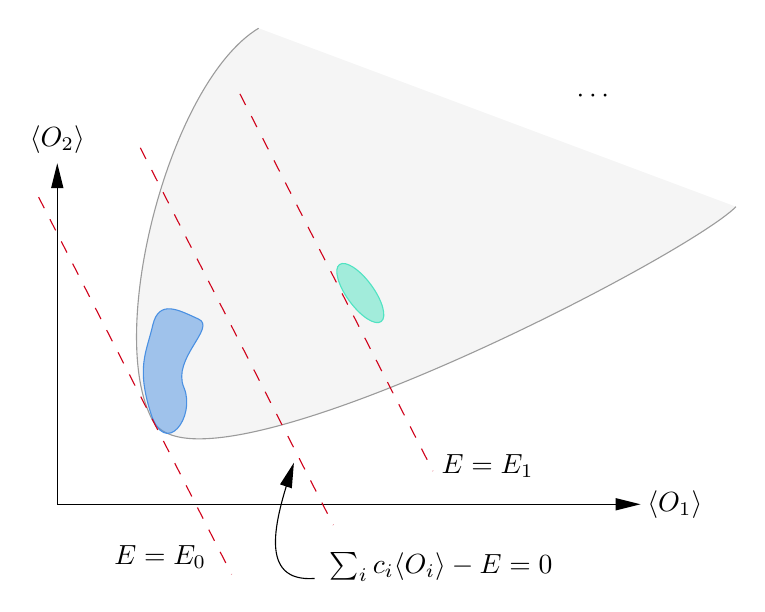
\begin{tikzpicture}[x=0.75pt,y=0.75pt,yscale=-1,xscale=1]
%uncomment if require: \path (0,353); %set diagram left start at 0, and has height of 353

%Curve Lines [id:da34254251114708456] 
\draw [color={rgb, 255:red, 155; green, 155; blue, 155 }  ,draw opacity=1 ][fill={rgb, 255:red, 155; green, 155; blue, 155 }  ,fill opacity=0.1 ]   (274,16.64) .. controls (231,42.64) and (200,163.64) .. (223,205.64) .. controls (246,247.64) and (479,127.64) .. (504,102.64) ;
%Straight Lines [id:da904255078328454] 
\draw    (177,246) -- (456,246) ;
\draw [shift={(458,246)}, rotate = 180] [fill={rgb, 255:red, 0; green, 0; blue, 0 }  ][line width=0.08]  [draw opacity=0] (12,-3) -- (0,0) -- (12,3) -- cycle    ;
%Straight Lines [id:da28860077544833507] 
\draw    (177,246) -- (177,83.73) ;
\draw [shift={(177,81.73)}, rotate = 90] [fill={rgb, 255:red, 0; green, 0; blue, 0 }  ][line width=0.08]  [draw opacity=0] (12,-3) -- (0,0) -- (12,3) -- cycle    ;
%Shape: Polygon Curved [id:ds05129166801576668] 
\draw  [color={rgb, 255:red, 74; green, 144; blue, 226 }  ,draw opacity=1 ][fill={rgb, 255:red, 74; green, 144; blue, 226 }  ,fill opacity=0.5 ] (223,159.73) .. controls (226,146.73) and (236,152.73) .. (245,156.73) .. controls (254,160.73) and (232,175.73) .. (238,189.73) .. controls (244,203.73) and (229,224.27) .. (222,202) .. controls (215,179.73) and (220,172.73) .. (223,159.73) -- cycle ;
%Straight Lines [id:da6483527344854445] 
\draw [color={rgb, 255:red, 208; green, 2; blue, 27 }  ,draw opacity=1 ] [dash pattern={on 4.5pt off 4.5pt}]  (168,98) -- (261,279.73) ;
%Straight Lines [id:da0036541181567224523] 
\draw [color={rgb, 255:red, 208; green, 2; blue, 27 }  ,draw opacity=1 ] [dash pattern={on 4.5pt off 4.5pt}]  (217,74.27) -- (310,256) ;
%Straight Lines [id:da34767057063343554] 
\draw [color={rgb, 255:red, 208; green, 2; blue, 27 }  ,draw opacity=1 ] [dash pattern={on 4.5pt off 4.5pt}]  (265,48.27) -- (358,230) ;
%Shape: Ellipse [id:dp302165402812995] 
\draw  [color={rgb, 255:red, 80; green, 227; blue, 194 }  ,draw opacity=1 ][fill={rgb, 255:red, 80; green, 227; blue, 194 }  ,fill opacity=0.5 ] (312.97,130.5) .. controls (310.07,132.62) and (312.21,140.48) .. (317.75,148.06) .. controls (323.29,155.64) and (330.13,160.08) .. (333.03,157.96) .. controls (335.93,155.84) and (333.79,147.98) .. (328.25,140.4) .. controls (322.71,132.81) and (315.87,128.38) .. (312.97,130.5) -- cycle ;
%Curve Lines [id:da7414078371933952] 
\draw    (301,281.73) .. controls (273.56,283.69) and (281.65,253.87) .. (290.46,227.6) ;
\draw [shift={(291,226)}, rotate = 108.67] [fill={rgb, 255:red, 0; green, 0; blue, 0 }  ][line width=0.08]  [draw opacity=0] (12,-3) -- (0,0) -- (12,3) -- cycle    ;

% Text Node
\draw (460,246) node [anchor=west] [inner sep=0.75pt]    {$\langle O_{1} \rangle $};
% Text Node
\draw (177,78.33) node [anchor=south] [inner sep=0.75pt]    {$\langle O_{2} \rangle $};
% Text Node
\draw (307,268) node [anchor=north west][inner sep=0.75pt]    {$\sum _{i} c_{i} \langle O_{i} \rangle -E=0$};
% Text Node
\draw (250,264.73) node [anchor=north east] [inner sep=0.75pt]   [align=left] {$\displaystyle E=E_{0}$};
% Text Node
\draw (360.97,234.5) node [anchor=south west] [inner sep=0.75pt]   [align=left] {\textcolor[rgb]{0,0,0}{$\displaystyle E=E_{1}$}};
% Text Node
\draw (426,45.4) node [anchor=north west][inner sep=0.75pt]    {$\cdots $};


\end{tikzpicture}

    \caption{线性SDP和非线性SDP:蓝色和绿色区域是非线性SDP的可行域,蓝色区域近似给出基态$E_0$上的物理量期望值,绿色区域近似给出基态$E_1$上的物理量期望值,灰色区域是线性SDP问题的可行域,虚线代表不同$E$对应的$\sum_i c_i \expval{O_i} = E$超平面,其中$c_i$为哈密顿量$H = \sum_i c_i O_i$的系数。}
    \label{fig:feasibility-compare}
\end{figure}

虽然非线性SDP能够让我们看清楚系统的激发态结构,目前尚无足够成熟的非线性求解器能够求解物理上需要的非线性SDP问题\cite{kazakov2021analytic}。
已报道的非线性SDP均仅限于单粒子量子力学,通过递推关系,将所有物理量约化至$E$和$\expval*{x^2}$上,然后暴力搜索\cite{han_matrix,bhattacharya2021}。

相比于同样基于最优化的变分法(包括各种张量网络方法),数值bootstrap有一个独特的优势:只要优化能够正确完成,它能够确定系统能量的\emph{下界}。
这是因为体系的各个物理量期望值必定让\eqref{eq:h-constraint},\eqref{eq:sym-constraint}和正定性条件成立,即一定在SDP问题的可行域当中,而数值bootstrap给出的能量数值值为可行域中的$\expval{H}$的\emph{最小值}。
因此,数值bootstrap给出的能量数值值必定小于等于能量真实值。
传统的最优化方法给出的则是能量的\emph{上界}。相互比较两种方法的结果,可以将系统基态能量的可能范围确定得非常小。

实际上,在使用传统方法得到能量上界之后,我们还能够进一步确定能量以外的物理量的上下界\cite{han_manybody}。设$E_\text{lb}$是通过bootstrap方法确定的能量下界,而$E_\text{ub}$是通过张量网络方法获得的能量上界,则真实的基态密度矩阵给出的$\expval{H}$显然在这两者之间,即$\rho_0$在集合
\[
    \{ \rho | \trace \rho = 1, \quad E_\text{lb} \leq \expval*{H}_\rho \leq E_\text{ub} \}
\]
中,于是,物理量$O$的基态期望值上下界由
\begin{equation}
    \min_{E_\text{lb} \leq \expval*{H}_\rho \leq E_\text{ub}} \expval{O}_\rho \leq \expval*{O}_{\rho_0} \leq \max_{E_\text{lb} \leq \expval*{H}_\rho \leq E_\text{ub}} \expval{O}_\rho
    \label{eq:operator-bound}
\end{equation}
给出。

\subsection{数值bootstrap的若干应用}

由于bootstrap不依赖于哈密顿量中各项的大小,它显然是处理非微扰问题的有力武器。
已有若干关于不同体系的数值bootstrap研究出现,涉及的体系包括难以微扰解决的单粒子量子力学问题和矩阵模型\cite{han_matrix,bhattacharya2021,kazakov2021analytic}以及强关联电子模型\cite{han_manybody}。

文献\parencite{bhattacharya2021}使用了以$E$和$\expval*{x^2}$为优化变量、暴力搜索的单粒子量子力学非线性SDP,捕捉到了二势阱模型中的非微扰瞬子效应,并与通过稀薄瞬子假设计算出的基态能量比较,直观展示了稀薄瞬子假设的成立条件;验证了互为对偶的超对称量子力学哈密顿量的谱的确是一致的;验证了$O(N)$向量模型的低能部分在强耦合极限下,基态能量和耦合常数的分数幂次关系,并确认其与解析结果一致。
\parencite{kazakov2021analytic}开发了一套处理矩阵模型的数值bootstrap中的矩阵自由度在大$N$极限下满足的非线性约束
\begin{equation}
    \left\langle\operatorname{Tr} M^{l} \operatorname{Tr} M^{m}\right\rangle=\left\langle\operatorname{Tr} M^{l}\right\rangle\left\langle\operatorname{Tr} M^{m}\right\rangle+\mathcal{O}\left(1 / N^{2}\right)
\end{equation}
的方法,验证了它在求解可以解析处理的矩阵模型时的有效性,并借此解决了无法解析处理的一类二矩阵矩阵模型。%
\footnote{这套方法对非线性SDP的作用可能有限,因为此时\eqref{eq:nonlinear-energy}和\eqref{eq:target-function}联立将导致任意高幂次的非线性约束,而矩阵模型中由于矩阵自由度的非线性约束幂次最多到2。}%
文献\parencite{han_manybody}将线性SDP数值bootstrap技术应用在一维和二维Hubbard模型上,所得结果和常规的DQMC、DMRG等方法吻合。

\section{关于本文}

本文在\prettyref{chap:oscillator}中复现了\parencite{han_matrix}的工作,分别在\prettyref{sec:nonlinear-sdp-oscillator}和\prettyref{sec:linear-sdp-oscillator}中使用非线性SDP和线性SDP方法求解了非简谐振子,并用定态薛定谔方程做基准测试。
非简谐振子可以通过常规的求解薛定谔方程的方法容易地解决,同时又是一个典型的非微扰系统,因此非常适合用作非微扰方法的玩具模型。
线性SDP、非线性SDP、定态薛定谔方程求解三者的结果互相对照,表明数值bootstrap技术能够非常精确地定量分析非简谐振子。

\prettyref{chap:hubbard}章复现了\parencite{han_manybody}的工作,使用线性SDP方法求解一维和二维Hubbard模型,并使用DMRG和一维Hubbard模型的精确解做了基准测试。Hubbard模型是最为简单的强关联电子模型,是各种量子多体方法的首选测试目标。
计算结果表明,对无掺杂,即一个格点平均有一个电子的Hubbard模型,数值bootstrap可以在不同大小的$U$下较为精确地计算双占据期望值并给出基态能量下界,在$U$较大时,精度更好,可能是由于此时电子巡游性不强,使用较为局域的算符能够较好地捕捉电子的行为。
对空穴掺杂的情况,数值bootstrap的精度有所下降,可能同样是因为此时电子巡游性较强。

最后,\prettyref{chap:future}总结了本文取得的进展以及遇到的问题,并展望了未来可能的研究方向,包括非简谐振子的线性SDP的收敛性问题、在更多的模型上实施数值bootstrap、如何更为经济地选取算符空间和约束、如何扩大计算规模等。

\chapter{一维非简谐振子的数值bootstrap}\label{chap:oscillator}

\section{一维非简谐振子——一个$0+1$维非微扰场论}

一维非简谐振子
\begin{equation}
    H = p^2 + x^2 + g x^4
\end{equation}
可以看成一个$0+1$维的$\phi^4$量子场论。它常常被用作量子力学中微扰论的例子,但实际上可以证明,其基态能量的微扰级数是发散的\cite{PhysRev.184.1231}。
这个发散可以看成$\phi^4$量子场论中的发散的一个特例。大部分量子场论中,相互作用均导致的微扰级数在最好的情况下也是渐进级数\cite{Jackiw_effective}。%
\footnote{此处所说的是朴素地将物理量展开成关于耦合常数$g$的幂次的级数后,会发现这个级数不收敛。在量子场论中这个级数的每一项都可能不收敛,因为动量积分时发生紫外发散。后一种不收敛和此处的讨论没有直接关系。
然而,\emph{重整化微扰论}——在微扰级数中引入抵消项,物理地看,是使用修饰后的耦合常数取代裸的耦合常数——可以用于消除紫外发散,并且可以在非简谐振子中重复,它在非简谐振子中的收敛性确实在\parencite{Bender-1970uz}中讨论过,结论是,很不幸,它仍然是发散的。}

由于一维非简谐振子归根到底是一个量子力学模型,可以通过求解离散定态薛定谔方程的方法精确地处理它。
它和$3+1$维多体问题的相似性又意味着,用于一般的多体问题的方法也可以用在它上面。
一维非简谐振子的简单形式和它的非微扰本质意味着它是测试多体问题研究方法的一个理想的玩具模型:可以通过比较这些数值或是解析方法和求解离散定态薛定谔方程的结果来预计这些方法的有效性,并分析这些方法为何有效或无效。
一维非简谐振子已被做大量不同的话题的例子,包括泛函重整化群\cite{Nagy-2010fv}、Rayleigh-Schrödinger微扰论的高阶行为\cite{bender199041}、重整化微扰论的收敛性\cite{Bender-1970uz}、量子多尺度分析\cite{Bender_1996}。

\section{非线性SDP优化}\label{sec:nonlinear-sdp-oscillator}

本节我们复现文献\parencite{han_matrix}中对非简谐振子
\begin{equation}
    H = p^2 + x^2 + g x^4
    \label{eq:anharmonic-hamiltonian}
\end{equation}
的非线性SDP计算。由于空间反演不变性,可以确认$n$为奇数时$\expval*{x^n} = 0$。
我们将正规序算符基底$\{O_i\}$选取为$\{x^{2n}\}, n \leq K$。
为此,有必要在不同的$\expval*{x^{2n}}$期望值之间建立非线性递推关系,最终将$n \geq 2$时的所有期望值都转化为能量期望值$E$和$x$的二阶矩$\expval*{x^2}$的多项式。
建立这种递推关系之后,根据矩阵
\begin{equation}
    M_{ij} = \expval*{x^{i + j}}
\end{equation}
的半正定性,即可得到$E$和$\expval*{x^2}$的范围。
由于此时独立的优化变量只有$E$和$\expval*{x^2}$,可以直接通过暴力搜索完成bootstrap。
我们使用Mathematica的\texttt{FindMinimum}函数即可完成整个计算流程。

\subsection{$\expval{x^n}$的非线性递推关系}

本节我们展示如何导出\parencite{han_matrix}中的方程(6)。根据$\expval*{OH} = E \expval*{O}$以及\eqref{eq:anharmonic-hamiltonian},并取$O = x^{t-1}$,我们有
\begin{equation}
    E \expval*{x^{t-1}} = \expval*{x^{t-1} p^2} + \expval*{x^{t+1}} + g \expval*{x^{t+3}}.
    \label{eq:e-h-o-constraint-oscillator}
\end{equation}
上式中出现了$p$的依赖,这会导致递推关系不封闭;此外,$E$也包含$\expval*{p^2}$的期望值。我们需要设法寻找一个包含$\expval*{x^{t-1} p^2}$和$\langle x^n \rangle$的递推关系。

$E$的期望值中的$\expval*{p^2}$可以通过在$\expval*{\comm{O}{H}} = 0$中取$O = xp$而消去。
我们有
\[
    \comm{p^2}{xp} = p \underbrace{[p, xp]}_{= [p, x] p = - \ii p} + [p, xp] p = - \ii p^2 - \ii p ^2 = - 2 \ii p^2,
\]
\[
    \comm{x^2}{xp} = x\comm{x^2}{p} = x \cdot (2 \ii x) = 2 \ii x^2,
\]
\[
    \comm{x^4}{xp} = x \comm{x^4}{p} = x \cdot (4 \ii x^3) = 4 \ii x^4,
\]
于是约束$\expval*{\comm{O}{H}} = 0$意味着
\[
    - 2 \ii \expval*{p^2} + 2 \ii \expval*{x^2} + 4 g \ii \expval*{x^4} = 0,
\]
于是
\begin{equation}
    \begin{aligned}
        E &= \expval*{p^2} + \expval*{x^2} + g \expval*{x^4} \\
        &= \expval*{x^2} + 2 g \expval*{x^4} + \expval*{x^2} + g \expval*{x^4} = 2 \expval*{x^2} + 3 g \expval*{x^4}.
    \end{aligned}
    \label{eq:e-x-2-x-4}
\end{equation}

我们仍然需要计算一般的$\expval*{x^{t-1} p^2}$。显然,通过在$\expval*{\comm{O}{H}} = 0$中取$O = x^t p$,由于
\[
    \begin{aligned}
        \comm{x^t p}{p^2} &= p \comm{x^t p}{p} + \comm{x^t p }{p} p = p \comm{x^t}{p} p + \comm{x^t}{p} p^2 \\
        &= p \ii t x^{t - 1} p + \ii t x^{t - 1} p^2 = \ii t (\comm{p}{x^{t-1}} p + 2 x^{t-1} p^2) \\
        &= \ii t (- \ii (t - 1) x^{t - 2} p + 2 x^{t-1} p^2) \\
        &= t(t-1) x^{t-2} p + 2 \ii t x^{t-1} p^2,
    \end{aligned}
\]
我们可以在得到的约束条件中看到一个$x^{t-1} p^2$项,但是同样出现了$x^{t-2} p$项,而这个项在\eqref{eq:e-h-o-constraint-oscillator}中是没有出现的。
因此,我们需要另一个只关于$\langle x^n p \rangle$和$\expval*{x^m}$的约束来消去这个项。
这样的约束是容易得到的:注意到
\[
    \begin{aligned}
        \comm{x^s}{p^2} &= p \comm{x^s}{p} + \comm{x^s}{p} p = p \cdot \ii s x^{s-1} + \ii s x^{s-1} p \\
        &= \ii s ( 2 x^{s-1} p + \comm{p}{x^{s-1}} ) = \ii s (2 x^{s-1} p - \ii (s-1) x^{s-2}) \\
        &= 2 \ii s x^{s-1} p + s (s-1) x^{s-2},
    \end{aligned}
\]
而$x^s$和$H$中关于$x$的项当然是对易的。于是$O= x^s, x^t p$的$\expval*{\comm{O}{H}} = 0$约束即可得到将$\expval*{x^{t-1} p^2}$和$\expval*{x^n}$的关系。
$O = x^s$的约束条件我们已经得到,它是
\begin{equation}
    0 = \expval*{\comm{x^s}{H}} = \expval*{\comm{x^s}{p^2}} = 2 \ii s \expval*{x^{s-1} p} + s (s-1) \expval*{x^{s-2}}.
    \label{eq:x-s-constraint}
\end{equation}
我们已经计算了$O = x^t p$和$p^2$的对易关系,它和$x^2, x^4$的对易关系分别是
\[
    \comm{x^t p}{x^2} = x^t \comm{p}{x^2} = x^t \cdot (- 2 \ii x) = - 2 \ii x^{t + 1},
\]
以及
\[
    \comm{x^t p}{x^4} = x^t \comm{p}{x^4} = x^t \cdot (- 4 \ii x^3) = - 4 \ii x^{t + 3}.
\]
这样$O = x^t p$给出的约束就是
\begin{equation}
    t(t-1) \expval*{x^{t-2} p} + 2 \ii t \expval*{t^{t-1} p^2} - 2 \ii \expval*{x^{t+1}} - 4 \ii g \expval*{x^{t+3}} = 0.
    \label{eq:x-t-p-constraint}
\end{equation}
在\eqref{eq:x-s-constraint}中代入$s=t-1$,并联立\eqref{eq:x-s-constraint}和\eqref{eq:x-t-p-constraint},消去$x^{t-2} p$,就得到
\[
    - t(t-1) \cdot \frac{t - 2}{2 \ii} \expval*{x^{t-3}} + 2 \ii t \expval*{x^{t-1} p^2} - 2 \ii \expval*{x^{t+1}} - 4 \ii g \expval*{x^{t+3}} = 0,
\]
即
\begin{equation}
    4 t \expval*{x^{t-1} p^2} = 4 \expval*{x^{t+1}} + 8 g \expval*{x^{t+3}} - t(t-1)(t-2) \expval*{x^{t-3}}.
\end{equation}
这就消去了\eqref{eq:e-h-o-constraint-oscillator}中的$\expval*{x^{t-1} p}$项,我们得到
\begin{equation}
    4 t E \expval*{x^{t-1}} + t(t-1)(t-2) \expval*{x^{t-3}} - 4 (t+1) \expval*{x^{t+1}} - 4g(t+2) \expval*{x^{t+3}} = 0.
    \label{eq:recursive-nonlinear-sdp-relation}
\end{equation}
这个递推关系中的$x^n$的期望值中,如果其中一个是偶数幂次的,那么全部都是偶数幂次的。在$E$和$\expval*{x^2}$给定后,根据\eqref{eq:e-x-2-x-4}可以计算出$\expval*{x^4}$,于是即可递推出$\expval*{x^6}, \expval*{x^8}, \ldots$,于是就能够构造出全部$\expval*{x^{2n}}$。
这样,即可将矩阵$M_{ij} = \expval*{x^{i+j}}$完全用两个变量$E$和$\expval*{x^2}$表示出来。

至此我们已经构造完成了关于非简谐振子的诸$\expval*{x^n}$的非线性SDP问题,它是
\begin{equation}
    \begin{aligned}
        &\min E, \quad \text{s.t.} \quad \expval*{x^n} = 0 \quad \text{for odd $n$}, \\
        &\quad M_{ij} = \expval{x^{i + j}}, \quad M \geq 0, \\
        &\quad E = 2 \expval*{x^2} + 3 g \expval*{x^4} , \\
        &\quad 4 t E \expval*{x^{t-1}} + t(t-1)(t-2) \expval*{x^{t-3}} - 4 (t+1) \expval*{x^{t+1}} - 4g(t+2) \expval*{x^{t+3}} = 0.
    \end{aligned}
    \label{eq:nonlinear-sdp-problem}
\end{equation}
在实际求解时,需要将$i$和$j$约束在范围
\begin{equation}
    0 \leq i, j \leq K
\end{equation}
中,$K$是对算符幂次上限的一个截断。

\subsection{可行域,基态和第一激发态}

我们在Mathematica中先为变量\texttt{g}赋值,然后执行以下代码:
\lstset{language=Mathematica,basicstyle=\small\ttfamily}
% Code from oscillator-simple-prototype/2022-1-20.nb
\begin{lstlisting}
    expectedX[0] := 1;
    expectedX[2] := x2;
    expectedX[4] := 1/(3 g) (E0 - 2 x2);
    expectedX[u_?EvenQ] := 1 / (4 g ((-3 + u) + 2)) * (
        4 (-3 + u) E0 expectedX[(-3 + u) - 1] 
        + (-3 + u) ((-3 + u) - 1) ((-3 + u) - 2) *
            expectedX[(-3 + u) - 3] 
        - 4 ((-3 + u) + 1) expectedX[(-3 + u) + 1]);

    matPositive[K_] := 
        Table[expectedX[i+j], {i, 0, K}, {j, 0, K}];
\end{lstlisting}
则函数\texttt{matPositive[K]}就给出了表示成变量\texttt{x2}(代表期望值$\expval{x^2}$)和变量\texttt{E0}(代表$E$;这里我们没有使用\texttt{E},因为Mathematica中符号\texttt{E}默认用于表示自然对数的底)的$M_{ij}$矩阵,参数\texttt{K}即为其幂次截断$K$。
之后,可以通过检查一个正方形区域内,不同的\texttt{E0}和\texttt{x2}值给出的\texttt{matPositive[K]}的特征值是否大于等于零,搜索得到非简谐振子的非线性SDP的可行域。
通过以下代码
\begin{lstlisting}
    RegionPlot[
        AllTrue[Eigenvalues[matPositive[9] /. g -> 1], 
        # >= 0 &], 
        {E0, 1.35, 1.44}, {x2, 0.294, 0.311}, 
    PlotPoints -> 100]
\end{lstlisting}
可以绘制$K$取为9时,$g=1$的非简谐振子(以下均取$g=1$)的非线性SDP可行域的一部分。比照通过其它手段获得的结果(见下一节),可以确定此处的可行域对应非简谐振子的基态。
通过以下代码
\begin{lstlisting}
    FindMinimum[{E0, 
        AllTrue[Eigenvalues[matPositive[9] /. g -> 1], # >= 0 &]}, 
        {{x2, 0.307}, {E0, 1.40}}]
\end{lstlisting}
可以计算给定$K$为9时的\texttt{E0}的极小值,以及此时\texttt{x2}的值。
注意,由于非线性SDP中,属于不同的能级的可行域经常是分散的,在使用\texttt{FindMinimum}寻找极小值点时需要指定初始值,初始值落在哪个能级的可行域中,\texttt{FindMinimum}就给出哪个能级的$E$和$\expval*{x^2}$估计值。

\begin{figure}
    \centering
    \begin{subfigure}{0.48\textwidth}
        \includegraphics[width=\textwidth]{nonlinear-oscillator-nonlinear-sdp-k-7-region.pdf}
        \subcaption{}
    \end{subfigure}
    \begin{subfigure}{0.48\textwidth}
        \includegraphics[width=\textwidth]{nonlinear-oscillator-nonlinear-sdp-k-7-8-9-region.pdf}
        \subcaption{}
    \end{subfigure}
    \caption{(a) 取$K$为7时的基态的$E$和$\expval{x^2}$的范围 (b) $K$为7, 8, 9时的基态的$E$和$\expval{x^2}$的范围}
    \label{fig:ground-state-e-x2-plot}
\end{figure}

\prettyref{fig:ground-state-e-x2-plot}是\texttt{RegionPlot}函数的输出,给出了非线性SDP问题\eqref{eq:nonlinear-sdp-problem}中不同$K$时的基态的$E$和$\expval{x^2}$的可行域。文献\parencite{han_matrix}的图1给出了几乎一样的图形,可以推测作者也是使用Mathematica完成的非线性SDP。
可以看到,随着$K$的增大,可行域快速缩小。实际上,当$K=9$时,可行域已经缩得如此之小,以至于\texttt{RegionPlot}的默认采样密度下,绘制出来的可行域是一片空白;需要将\texttt{PlotPoints}设置到至少100才能够绘制出正确的可行域。

类似的,如\prettyref{fig:first-excited-nonlinear-oscillator}所示,在第一激发态的能量附近做暴力搜索,同样可以发现一个可行域的连通分支。

\begin{figure}
    \centering
    \includegraphics[width=0.48\textwidth]{nonlinear-oscillator-nonlinear-sdp-k-10-first-excited-region.pdf}
    \caption{$K=10$时的第一激发态的$E$和$\expval{x^2}$的范围}
    \label{fig:first-excited-nonlinear-oscillator}
\end{figure}

% data from oscillator-simple-prototype/2022-1-20.nb

\begin{table}
    \caption{不同$K$下的非线性SDP结果}
    \label{tbl:nonlinear-different-k}
    \centering
    \begin{tabular}{ccc}
        \toprule
          $K$ & $E$ & $\expval*{x^2}$ \\
        \midrule
           7 & 1.3609004491049470  & 0.29816865118929264  \\
           8 & 1.3636216063227670  & 0.30113812134566936  \\
           9 & 1.3865039748817591  & 0.30434383991470115  \\
          10 & 1.3865039748792434  & 0.30434383991413540  \\ 
          11 & 1.3921989769203813  & 0.30578155266869480  \\
          12 & 1.3921989772554817  & 0.30578148147678430  \\
        \bottomrule
    \end{tabular}
\end{table}

\prettyref{tbl:nonlinear-different-k}给出了不同截断下的非线性SDP结果。观察可以发现,随着$K$的提升,基态能量计算结果呈现上升趋势,并且似乎在逐渐收敛。
这和\prettyref{sec:formalism}中所述的基态能量计算值是真实值的下界一致,也表明,通过扩大问题规模,可以系统地提升计算精度。

\subsection{定态薛定谔方程基准测试}

% data from oscillator-simple-prototype/stationary-schrodinger-2.jl

\begin{table}
    \caption{不同$\Delta x$下定态薛定谔方程的基态}
    \label{tbl:stationary-benchmark}
    \centering
    \begin{tabular}{ccc}
        \toprule
          $\Delta x$ & $E$ & $\expval*{x^2}$ \\
        \midrule
          0.1   & 1.3907396718070801  & 0.30534500159391625  \\
          0.05  & 1.3919487648892426  & 0.30569659174520486  \\
          0.02  & 1.3922871864425093  & 0.30579492589833174  \\
          0.01  & 1.3923355279431886  & 0.30580896967753670 \\ 
          0.005 & 1.3923476131451260  & 0.30581248046786375  \\
        \bottomrule
    \end{tabular}
\end{table}

为测试\prettyref{tbl:nonlinear-different-k}的可靠性,我们选择求解定态薛定谔方程来模拟非简谐振子。相应的薛定谔方程为
\begin{equation}
    - \laplacian \psi + x^2 \psi = E \psi, \quad \psi(x \to \pm \infty) = 0.
    \label{eq:schrodinger-oscillator}
\end{equation}
为了做数值求解,采用步长为$\Delta x$的有限差分格式,则$\laplacian$近似为一个矩阵,其中
\begin{equation}
    \laplacian_{i, i} = -2 / \Delta x^2, \quad \laplacian_{i, i - 1} = \laplacian_{i, i+1} = 1 / \Delta x^2,
\end{equation}
其余矩阵元为零,$\hat{x}$算符近似为一个对角矩阵,$x_{ii}$为$i$点的坐标。
进一步,将求解域限制在$- L \leq x \leq L$上。设求解域被离散化为$N$个点。在$L$充分大时,可以认为波函数在求解域的两端为零,于是在$i=1$和$i = N$时分别有
\begin{equation}
    \laplacian_{1, 1} = -2, \quad \laplacian_{1, 2} = 1, \quad \laplacian_{N, N} = -2, \quad \laplacian_{N, N-1} = 1.
\end{equation}
于是,$\laplacian$被截断为一个$N \times N$维矩阵。求解\eqref{eq:schrodinger-oscillator}等价于对角化矩阵$-\laplacian + x^2$。
我们采用Arpack-NG库(用于大型矩阵对角化的Arpack库的一个实现)\cite{arpackcode}的Julia封装Arpack.jl\cite{arpackjl}完成这项工作。取$L=10$以及不同的$\Delta x$,使用Arpack.jl计算$-\laplacian + x^2$的最低本征态,即系统基态,所得结果见\prettyref{tbl:stationary-benchmark}。
表中不同的$\Delta x$对应的波函数均平滑。
可以看到,\prettyref{tbl:nonlinear-different-k}和\prettyref{tbl:stationary-benchmark}给出的值非常接近。取两者中计算精度最高的值(\prettyref{tbl:nonlinear-different-k}中$K=12$和\prettyref{tbl:stationary-benchmark}中的$\Delta x = 0.005$),计算相对偏差,发现$E$的相对偏差为\num{1.1e-4},$\expval*{x^2}$的相对偏差为\num{1.0e-4},两者符合程度较好。

\subsection{计算$\langle x^m p^n \rangle$参考值}

\begin{figure}
    \centering
    \includegraphics[width=0.6\textwidth]{oscillator-expectations.pdf}
    \caption{非简谐振子的非线性SDP计算得到的$K=11$时的$\langle x^m p^n \rangle$参考值}
    \label{fig:oscillator-expectation}
\end{figure}

% calculate-all-correlation-functions-in-xp-oscillator-for-benchmark-4.nb
在已经获得了精度较高的$E$和$\expval*{x^2}$数据之后,我们可以据此计算所有$\expval*{x^m p^n}$值。
在Mathematica中直接列出所有的$\expval*{\comm{O}{H}} = 0$并使用\texttt{Solve}求解是非常缓慢的,采用如下方法可以较快地获得任意$m, n$的$\expval*{x^m p^n}$。
注意到,$x^n$和$H$的对易子就是$x^n$和$p^2$的对易子,其正规序形式$p$的次数最高为1;$x^n p$和$H$的对易子中$p$的次数最高的项由$x^n p$和$p^2$的对易子贡献,$p$的次数最高为2……如此重复,$x^m p^n$和$H$的对易子的正规排序形式中,$p$的次数最高为$n+1$。
因此,可以使用\eqref{eq:recursive-nonlinear-sdp-relation}计算出所有的$\expval*{x^m}$型期望值,然后使用这些数据连同$\expval*{\comm{H}{x^m}} = 0$给出的约束条件,计算出所有的$\expval*{x^m p}$型期望值,然后引入$\expval*{\comm{H}{x^m p}} = 0$型约束条件,计算所有的$\expval*{x^m p^2}$型期望值……如此重复,即可计算出次数小于某个截断的所有的$\langle x^m p^n \rangle$期望值。
\prettyref{fig:oscillator-expectation}展示了一些这样计算出的期望值。应注意,如果要使用这些数据做其它SDP程序的基准测试,必须取更多的小数点后位数。

\section{线性SDP优化}\label{sec:linear-sdp-oscillator}

本节讨论如何使用线性SDP实施非简谐振子的数值bootstrap。在\prettyref{sec:nonlinear-sdp-oscillator}中,我们能够分析第一激发态处的物理量,而在线性SDP中我们只能讨论基态性质。
然而,由于非线性SDP在大规模问题上是不可行的(见\prettyref{sec:numerical-boostrap-intro}的讨论),线性SDP对凝聚态体系基本上是唯一的选择。
因此,本节将非简谐振子当作一个玩具模型,用它演示如何做线性SDP,为在凝聚态体系中做数值bootstrap做准备。

\subsection{对易子和等式关系的符号计算}

非简谐振子线性SDP的问题可以叙述如下:设
\begin{equation}
    O_i^\dagger O_j = \sum_{k} c_{ij}^k O_k,
\end{equation}
\begin{equation}
    \comm{H}{O_i} = \sum_j h_j^k O_k,
\end{equation}
则我们有
\begin{equation}
    \begin{aligned}
        &\min E, \quad \text{s.t.} \quad E = \expval*{p^2} + \expval*{x^2} + g \expval*{x^4}, \\
        &\quad M_{ij} \coloneqq \sum_k c^k_{ij} \expval*{O_i}, \quad M \geq 0, \quad M_{ij} = M_{ji}^* , \\
        &\quad \sum_j h_j^k \expval*{O_k} = 0.
    \end{aligned}
    \label{eq:oscillator-linear-sdp}
\end{equation}
注意,在以上问题中,$\expval*{O_i}$应该\emph{整体}当成一个优化变量;线性SDP求解器不关心它是否是某个物理量的期望值。
约束条件$M_{ij} = M_{ji}^*$保证了$\expval*{O^\dagger} = \expval*{O}^*$。

使用$\{x^m p^n\}$满足$0 \leq m, n \leq L$的子集,按照$\expval*{O_i^\dagger O_j}$的方法构建$M$矩阵。
这可以保证$\{x^m p^n\}$中的每个算符都出现在$M$矩阵中,不至于浪费优化变量。
显然,$M$矩阵的边长为$(L+1)^2$。

此时没有类似\eqref{eq:recursive-nonlinear-sdp-relation}这样较为精简的递推公式,$c_{ij}^k$和$h_j^k$的计算需要计算机来完成。
我们取$\{O_i\}$为$\{x^m p^n\}$,并将其张成的空间设为$\mathcal{C}$。我们对$\{x^m p^n\}$施加如下截断:要求
\begin{equation}
    0 \leq m, n \leq 2 L,
\end{equation}
其中$L$是一个正整数。我们将$x^m p^n$算符编号为$m(2L+1) + n$,这样,基底$\{x^m p^n\}$的编号就从0一直连续取到$(2L+1)^2-1$,$\mathcal{C}$是一个$(2L+1)^2$维的线性空间。
我们有McCoy公式\cite{McCoyOnCF}
\begin{equation}
    {\left[{ {x}}^{n},{ {p}}^{m}\right]=\sum _{k=1}^{\min \left(m,n\right)}{{\frac {-\left(-i\hbar \right)^{k}n!m!}{k!\left(n-k\right)!\left(m-k\right)!}}{ {x}}^{n-k}{ {p}}^{m-k}}},
\end{equation}
将这个公式代入
\begin{equation}
    {x^{m_1} p^{n_1}}{x^{m_2} p^{n_2}} = x^{m_1 + m_2} p^{n_1 + n_2} - x^{m_1} \comm{x^{m_2}}{p^{n_1}} p^{n_2}
    \label{eq:oscillator-normal-ordering-scheme}
\end{equation}
等式右边就已经是正规排序的了。于是,可以实现一个函数 \texttt{xpopstr\_normal\_ord} ,输入$m_1, n_1, m_2, n_2$,输出\eqref{eq:oscillator-normal-ordering-scheme}右边在基底$\{x^m p^n\}$下的系数。于是,我们就能够自动计算$p^{n_1} x^{m_1} x^{m_2} p^{n_2}$,于是$c^k_{ij}$即可自动计算。
通过将${x^{m_1} p^{n_1}}{x^{m_2} p^{n_2}}$和${x^{m_2} p^{n_2}}{x^{m_1} p^{n_1}}$的系数向量相减,$\comm{O_1}{O_2}$的系数向量也可以自动计算,于是$h^k_j$也可以自动计算。
这就给出了基底$\{x^m p^n\}$下自动计算$h_j^k$和$c^k_{ij}$的方法。
注意,对一些$\mathcal{C}$中的$O$,$\comm{O}{H}$可能在$\mathcal{C}$外,此时我们丢弃它对应的等式约束。

\subsection{构建优化问题}

我们使用JuMP 0.22.3\cite{DunningHuchetteLubin2017}和COSMO 0.8.5\cite{Garstka_2021}构建并求解优化问题\eqref{eq:oscillator-linear-sdp}。
JuMP是一个优化器前端,可以通过\eqref{eq:oscillator-linear-sdp}这样的记号,高可读性地构建优化问题,而无需手动将\eqref{eq:oscillator-linear-sdp}中的约束组装成系数矩阵再传给优化器。
COSMO是一个大规模凸优化问题求解器,适用于线性SDP问题。

由于COSMO不支持复数变量,在构建优化问题时需要将$\langle x^m p^n \rangle$的实部和虚部声明为不同的变量。
注意到在一维束缚态问题中,如果$m+n$是奇数,那么$\expval*{x^m p^n} = 0$,否则,如果$m$是偶数,那么$\expval*{x^m p^n}$是纯实数,如果$n$是奇数,那么$\expval*{x^m p^n}$是纯虚数。
因此,可以只对$m+n$为偶数的那些$\expval*{x^m p^n}$声明优化变量,且对每个期望值只声明一个变量,代表其实部或虚部。

在声明完优化变量之后,可以使用JuMP提供的\texttt{@constraint}宏,对这些变量施加\eqref{eq:oscillator-linear-sdp}中由$h_j^k$确定的那些约束。

由于\eqref{eq:oscillator-linear-sdp}中的$M$矩阵包含复数,在JuMP中构建优化问题时,需要把它的每一个矩阵元$M_{ij}$替换为
\begin{equation}
    \Re(M_{ij}) \pmqty{1 & 0 \\ 0 & 1} + \Im(M_{ij}) \pmqty{0 & -1 \\ 1 & 0}.
    \label{eq:complex-to-real}
\end{equation}
我们可以在JuMP中声明一个边长为$2(L+1)^2$的半正定矩阵变量,然后使用\texttt{@constraint}宏将$M_{ij}$和$\{\expval*{O_i}\}$联系起来。
由于在大部分线性SDP求解器中,被声明为半正定的矩阵变量一定是对称的%
\footnote{可以运行几次迭代,然后用\texttt{value.(M)}检查此时的\texttt{M}的值。计算其本征值,会发现有绝对值很小的负值,但是比较它和它的转置,会发现两者完全相同。}%
,将$M_{ij}$的每个矩阵元都和$\{\expval*{O_i}\}$联系起来之后,$\expval*{O^\dagger} = \expval*{O}^*$的约束就自动被施加了。

\subsection{使用非线性SDP为线性SDP做基准测试}\label{sec:oscillator-benchmark}

由于已经有了非线性SDP计算出的数据,非简谐振子线性SDP程序的调试将变得容易很多,因为可以直接检查非线性SDP的计算结果是否满足线性SDP程序中的各种约束,从而检查程序是否正确。

在完成线性SDP的程序开发后,使用\texttt{primal\_feasibility\_report}函数可以检查一个特定的数据点是否在可行域中,以及如果不在可行域中,各个约束被违反了多少。
我们可以将Mathematica中的计算结果\prettyref{fig:oscillator-expectation}导出为一个Julia的\texttt{Dict}对象,将它传给\texttt{primal\_feasibility\_report}。
结果发现,在$L=5$时,等式约束被违反的数值的量级是\num{1e-11},其主要来源是导出数据时的舍入误差。
% 见oscillator-simple-prototype/labbook.md的2022.3.26的记录
目前JuMP和COSMO尚未配合得足够好,无法直接通过\texttt{primal\_feasibility\_report}检查$M$矩阵的半正定性,但是直接根据\prettyref{fig:oscillator-expectation},在线性SDP程序中计算$M$矩阵,发现$L=5$时,它有负本征值,但其量级最大在\num{6e-3},而最大的本征值量级为\num{1e5},于是可以认为线性SDP程序对M矩阵的计算也是正确的。

\subsection{计算结果与收敛性问题}\label{sec:convergence-problem}

% data from oscillator-simple-prototype/jump-oscillator-4-small-scale.jl

\begin{table}
    \caption{不同$L$下的线性SDP计算结果}
    \label{tbl:linear-sdp-oscillator-result}
    \centering
    \begin{tabular}{cccc}
        \toprule
          $L$ & $E$ & $\expval*{x^2}$ & 耗时 \\
        \midrule
          2 & 1.3810167562983844  & 0.3131420484955468 & 0.752s  \\
          3 & 1.3896818143288878  & 0.3054621206463042 & 2.501s  \\
          4 & ?  & ?& ?  \\
        \bottomrule
    \end{tabular}
\end{table}

$L = 2, 3, 4$时的线性SDP计算结果见\prettyref{tbl:linear-sdp-oscillator-result}。%
\footnote{本例中使用的代码见\url{https://github.com/wujinq/numerical-boostrap/blob/main/oscillator-simple-prototype/jump-oscillator-4-small-scale.jl}。}%
可以看到,在$L=2, 3$时,使用非常短的时间,线性SDP就能够达到\prettyref{tbl:nonlinear-different-k}中$K=10$的精度。
在联想T480笔记本电脑上,$L=10$的非线性SDP需要耗费几分钟,而线性SDP只需要两秒,体现了SDP求解器相对暴力搜索的巨大优势。

% 见2022.4.27的oscillator-simple-prototype\labbook.md
然而,$L=4$时,存在严重的收敛性问题。COSMO的默认容差(线性约束被违反的程度——见COSMO的文档\parencite{cosmo-method})无法达到要求的精度:程序运行至19698迭代后,能量达到25.31,提示收敛。
% 见2022.3.22的oscillator-simple-prototype\labbook.md
$L=5$时COSMO的默认容差同样无法达到要求的精度:在经过漫长的3353517次迭代之后,程序运行到能量约为13.9,提示收敛。
% 见2022.4.20的oscillator-simple-prototype\labbook.md
改用CSDP求解器,会提示“Lack of progress”;SCS求解器直接报告问题不可解。

% 见2022.4.29的oscillator-simple-prototype\labbook.md
将容差参数\texttt{eps\_rel}从默认值\num{1e-5}缩小至\num{1e-10},$L=4$时的线性SDP能够收敛,但是耗时增长高得可观。
检查优化器输出,发现与$L=2, 3$时的优化器输出相比,至少存在以下几个不同。$L=4$时,需要约50000迭代让能量到达10左右,在此之前会经历能量上百的阶段,而$L=2, 3$时没有这种情况,能量只需要25迭代就到达了非简谐振子的基态能量的量级。
$L=2, 3, 4$的问题中,均有出现能量振荡的现象,这本身是正常的,因为大规模求解器不会施加硬约束,半正定约束和线性约束都是通过向目标函数引入柔化的指示函数完成的\cite{cosmo-method},因此,一个让能量下降的优化过程很可能以轻微违反各种约束为代价,后续收紧约束的优化过程当然也可能会让能量上升。然而,在$L=4$的优化过程中,会出现非常长周期的能量振荡:可能出现几万个迭代的能量上升,然后是一段能量下降的过程,接着又是长时间的能量振荡。
在能量已经接近目标时,优化过程非常慢。例如,7000000迭代时,能量已经到达1.54,然而还要经过比这多一个量级的迭代数目才能够最终收敛。
推测这也是加细约束过程中的能量振荡导致的,只不过振荡的量级小于\num{1e-4},没有在优化器输出中显示。

% 见2022.4.7的oscillator-simple-prototype\labbook.md
将容差参数\texttt{eps\_rel}从默认值\num{1e-5}缩小至\num{1e-10}后,$L=5$时的线性SDP未能完成。在经过了80000000个迭代之后,能量到达5.3690,此时系统能量仍然在前述和收紧约束有关的缓慢振荡中。

在共形bootstrap中,常规的64位浮点数有时无法满足精度要求,即舍入误差可能在计算过程中放大,导致一个点是否在可行域中无法正确判断,从而大小合理的容差难以达到;放松容差要求,则可能出现优化不充分的情况。
因此,支持任意精度的优化算法是必要的\cite{conformal-sdp}。为了检查是否在本例中出现了这种情况,而可以将$L=2, 3$的优化问题中的浮点数精度人为调小,观察计算收敛性。
不幸的是,JuMP目前不支持调整浮点数精度%
\footnote{见此处的讨论:\url{https://discourse.julialang.org/t/use-low-precision-float-type-in-jump/80332}。}%
,因此眼下调整浮点数精度需要将代码重写为稍微低层一些的MathOptInterface\cite{legat2021mathoptinterface}代码,由于时间因素,非简谐振子的线性SDP中的收敛性问题来自何处的讨论只能留给未来的研究了。

\chapter{Hubbard模型的数值bootstrap}\label{chap:hubbard}

\section{Hubbard模型简介}

本章讨论Hubbard模型
\begin{equation}
    H = - t \sum_{\pair{\vb*{i}, \vb*{j}}, \sigma} c^\dagger_{\vb*{i} \sigma} c_{\vb*{j} \sigma} + U \sum_{\vb*{i}} n_{\vb*{i} \uparrow} n_{\vb*{j} \downarrow}
\end{equation}
的线性SDP数值bootstrap。Hubbard模型是一个格点强关联电子模型,描述了一个声子作用可忽略,费米面附近只有一条可以使用紧束缚模型描述的能带,原位(on-site)库伦排斥最为重要,长距离库伦排斥不重要的系统。
在能带半填充,$U$较大时,Hubbard模型退化为海森堡模型,其中电子定域而无法自由移动,从而电荷自由度(即电子数自由度)不再是低能自由度,只有每个格点上的自旋自由度是基本自由度。
从能带论的角度,这可以理解为强烈的相互作用导致出现能带劈裂,费米能级落在禁带上,从而体系成为Mott绝缘体。
因此,Hubbard模型对铁磁学显然非常重要。
此外,掺杂(从而费米能级位置发生变动)的Hubbard模型可能能够从完全的排斥相互作用出发产生电子配对,从而也是高温超导的可能机制之一。
总之,Hubbard模型的简单性以及它的丰富物理含义让它成为了研究强关联电子系统的基础\cite{fradkin2013field}。

DMRG方法可以在开边界条件下以相当高的精度计算各种一维强关联格点系统\cite{Schollw_ck_2011},
此外,使用Bethe拟设可以严格求解一维Hubbard模型以及其它若干强关联电子模型\cite{PhysRevLett.20.1445,korepin1994exactly}。
这些工作使得一维Hubbard模型成为了测试量子多体方法适用性的理想玩具模型。一维Hubbard模型也可以用于粗略地复现一维铜基超导体$\mathrm{Sr}_{2} \mathrm{CuO}_{3}$链、聚二乙炔等一维系统,虽然已知的类似Hubbard模型的系统往往涉及不止一条能带(由于Peierls转变),并且重要的库仑相互作用通道不仅仅有原位库伦排斥。
在\prettyref{sec:one-dimensional-hubbard}中,我们尝试复现\parencite{han_manybody}中关于一维Hubbard模型的部分。

二维Hubbard模型的数值研究具有更加直接的物理意义(例如,它的相图和铜基超导体类似,在掺杂时存在赝能隙\cite{2d-hubbard-numerical}),也更具挑战性。一些二维系统——包括Hubbard模型——仍然可以使用DMRG方法非常有效地处理,但计算开销较大\cite{Stoudenmire_2012}。
朴素地对Hubbard模型做DQMC模拟会遇到符号问题,需要通过选择适当的基底等方式去除\cite{pgp-sign}。
我们在\prettyref{sec:hubbard-2d}中将讨论二维Hubbard模型的数值bootstrap。

\section{一维Hubbard模型的数值bootstrap}\label{sec:one-dimensional-hubbard}

\subsection{算符空间截断}

\begin{figure}
    \centering
    

\tikzset{every picture/.style={line width=0.75pt}} %set default line width to 0.75pt        

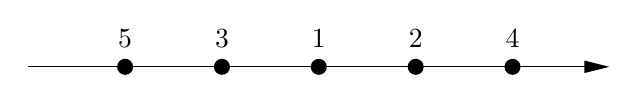
\begin{tikzpicture}[x=0.75pt,y=0.75pt,yscale=-1,xscale=1]
%uncomment if require: \path (0,300); %set diagram left start at 0, and has height of 300

%Straight Lines [id:da7449686192404181] 
\draw    (100,153) -- (146.67,153) ;
\draw [shift={(146.67,153)}, rotate = 0] [color={rgb, 255:red, 0; green, 0; blue, 0 }  ][fill={rgb, 255:red, 0; green, 0; blue, 0 }  ][line width=0.75]      (0, 0) circle [x radius= 3.35, y radius= 3.35]   ;
%Straight Lines [id:da9017019116760947] 
\draw    (146.67,153) -- (193.33,153) ;
\draw [shift={(193.33,153)}, rotate = 0] [color={rgb, 255:red, 0; green, 0; blue, 0 }  ][fill={rgb, 255:red, 0; green, 0; blue, 0 }  ][line width=0.75]      (0, 0) circle [x radius= 3.35, y radius= 3.35]   ;
%Straight Lines [id:da26753414986637103] 
\draw    (193.33,153) -- (240,153) ;
\draw [shift={(240,153)}, rotate = 0] [color={rgb, 255:red, 0; green, 0; blue, 0 }  ][fill={rgb, 255:red, 0; green, 0; blue, 0 }  ][line width=0.75]      (0, 0) circle [x radius= 3.35, y radius= 3.35]   ;
%Straight Lines [id:da9354128008118774] 
\draw    (240,153) -- (286.67,153) ;
\draw [shift={(286.67,153)}, rotate = 0] [color={rgb, 255:red, 0; green, 0; blue, 0 }  ][fill={rgb, 255:red, 0; green, 0; blue, 0 }  ][line width=0.75]      (0, 0) circle [x radius= 3.35, y radius= 3.35]   ;
%Straight Lines [id:da7011463755992022] 
\draw    (286.67,153) -- (333.33,153) ;
\draw [shift={(333.33,153)}, rotate = 0] [color={rgb, 255:red, 0; green, 0; blue, 0 }  ][fill={rgb, 255:red, 0; green, 0; blue, 0 }  ][line width=0.75]      (0, 0) circle [x radius= 3.35, y radius= 3.35]   ;
%Straight Lines [id:da5013137889897423] 
\draw    (333.33,153) -- (378,153) ;
\draw [shift={(380,153)}, rotate = 180] [fill={rgb, 255:red, 0; green, 0; blue, 0 }  ][line width=0.08]  [draw opacity=0] (12,-3) -- (0,0) -- (12,3) -- cycle    ;

% Text Node
\draw (240,145) node [anchor=south] [inner sep=0.75pt]   [align=left] {1};
% Text Node
\draw (286.67,145) node [anchor=south] [inner sep=0.75pt]   [align=left] {2};
% Text Node
\draw (193.33,145) node [anchor=south] [inner sep=0.75pt]   [align=left] {3};
% Text Node
\draw (333.33,145) node [anchor=south] [inner sep=0.75pt]   [align=left] {4};
% Text Node
\draw (146.67,145) node [anchor=south] [inner sep=0.75pt]   [align=left] {5};


\end{tikzpicture}

    \caption{一维简单晶格的格点编号方案}
    \label{fig:1d-lattice-index}
\end{figure}

我们遵从\parencite{han_manybody}中的做法,使用以下标准来截断算符空间:我们以正规排序的形如
\begin{equation}
    O = c^\dagger_{{x}_1 \sigma_1} c^\dagger_{x_2 \sigma_2} \cdots c^\dagger_{x_m \sigma_m} c_{x_{m+1} \sigma_{m+1}} \cdots c_{x_{n} \sigma_n}
    \label{eq:hubbard-operator-form}
\end{equation}
算符乘积为基底,只有满足
\begin{equation}
    l(O) \coloneqq n + \sum_{i=1}^n \left\| x_{i} \right\|_1 \leq K
    \label{eq:operator-space-criteria}
\end{equation}
的算符被纳入我们考虑的算符空间。为了避免重复计数,我们将每个格点赋予一个编号(见\prettyref{fig:1d-lattice-index};由于格点无限大,需要使用这种左一个右一个的方式编号),并且要求\eqref{eq:hubbard-operator-form}的产生算符和湮灭算符部分中,从左往右格点编号均依次增大。
这么定义正规排序的原因是这是后面做符号计算使用的QuantumAlgebra.jl包(见\prettyref{sec:symbolic-hubbard})定义正规排序的方法。可以通过如下代码验证这一点:
\begin{verbatim}
    julia> normal_form(c(1) * c(2))
    c(1) c(2)

    julia> normal_form(cdag(1) * cdag(2))
    c†(1) c†(2)
\end{verbatim}

注意到,由于$O = O_1 O_2$,我们有
\begin{equation}
    l(O) = l(O_1) + l(O_2),
\end{equation}
因此,可以首先构造出满足$l(O) \leq K$的所有湮灭算符乘积,然后将$c$替换成$c^\dagger$就得到了满足$l(O) \leq K$的所有产生算符乘积,两者的乘积中包含所有满足$l(O) \leq K$的产生湮灭算符乘积。
这就完成了截断过的算符空间的构造。

在构造满足$l(O) \leq K$的所有产生算符乘积时,我们当然不可能遍历无数个格点,也不能够遍历任意长的产生湮灭算符乘积,不过\eqref{eq:operator-space-criteria}显然意味着
\begin{equation}
    \max \| x_i \|_1 \leq K - 1, \quad n \leq K.
    \label{eq:inequality-hubbard-opstr}
\end{equation}
因此,可以如下搜索满足条件\eqref{eq:operator-space-criteria}的所有湮灭算符乘积:我们列出所有满足$\abs*{x_i} \leq K - 1$的格点$x_i$,在每个格点上放置如下四种状态之一:没有算符,有一个自旋向上的湮灭算符,有一个自旋向下的湮灭算符,同时有自旋向上和向下的湮灭算符,然后筛去不满足\eqref{eq:operator-space-criteria}的情况即可。
我们记所有满足此条件的算符构成的集合为$\mathcal{C}$,它张成的空间就是我们在bootstrap中考虑的算符空间。

\subsection{等式约束和半正定约束的构建}\label{sec:symbolic-hubbard}

我们使用QuantumAlgebra.jl 1.1.0包\cite{Sanchez-Barquilla2020,QuantumAlgebra.jl}自动完成费米子算符的对易关系和正规排序计算。
调用QuantumAlgebra.jl包,并调用\texttt{@fermion\_ops}宏声明湮灭算符\texttt{c}后,即可使用\texttt{c(args...)}和\texttt{cdag(args...)}两个函数得到标签为\texttt{args}的湮灭算符和产生算符。
根据\prettyref{fig:1d-lattice-index}为格点编号,并使用\texttt{1}表示自旋向上的算符,\texttt{-1}表示自旋向下的算符。
例如,取原点为1号格点,则$c^\dagger_{x = 1, \uparrow}$在程序中对应\texttt{cdag(2,1)}。%
\footnote{
    由于Julia支持unicode变量名,更加规范的做法本应是将自旋向上就使用$\uparrow$表示。然而,目前的QuantumAlgebra.jl版本将传递给它的标签中能够做合法的变量名(包括字符串)的东西都看成抽象的、值可变的指标,其结果是没有办法区分\texttt{cdag(i,↑)}和\texttt{cdag(i,↓)}。
    我们不得不使用整数来表示自旋标签(浮点数目前不受支持)。
}%

本例中的等式约束来自哈密顿量$H$、总自旋$S^z$、总粒子数$N$、平移对称性、空间反演对称性。前三个对称性导致的约束通过计算对易关系得到:我们构造一个容纳了$\mathcal{C}$中出现的所有格点的格子上的近似哈密顿量、总自旋、总粒子数,使得它们和$\mathcal{C}$中任何一个算符的对易子都等于后者和真正的$H, S^z, N$的对易子,然后使用QuantumAlgebra.jl包计算对易子即可。
平移对称性和空间反演对称性原则上也可以通过对易子计算得到,但是此处应注意,平移操作的生成元不是
\[
    \sum_{i, \sigma} c^\dagger_{i \sigma} c_{i + 1, \sigma},
\]
空间反演对称操作也不是
\[
    \sum_{i, \sigma} c^\dagger_{i \sigma} c_{-i, \sigma}.
\]
这两个算符和含有超过两个算符的产生湮灭算符乘积的对易子是不正确的。因此,直接修改QuantumAlgebra.jl算符上的格点标签,将5变成3,3变成1,1变成2……以及将3变成2,5变成4……然后计算格点变换前后的算符的差,是得到平移对称性约束和空间反演对称性约束方程的最简单的方法。

在完成所有对易关系和正则排序计算后,可以将其中的产生湮灭算符乘积替换为相应的JuMP优化变量。
与非简谐振子的情况不同,本例中所有算符期望值都是实的%
\footnote{
    在粒子数表象中思考问题即可看清楚这一点:无论是$c^\dagger_{i \sigma} c_{i + 1, \sigma}$还是$n_{i \uparrow} n_{i \downarrow}$都是实矩阵,哈密顿量中又不存在复数,因此整个哈密顿量都是实的,其本征值也是实的,并且$c^\dagger \cdots c^\dagger c \cdots c$也是实矩阵,从而其期望值也是实的。

    量子力学问题涉及不可数无穷维算符,因此一个实的哈密顿量完全可以有复的本征态——如平面波等散射态。
    即使束缚态波函数是实的,由于动量算符不是实的,不能保证算符空间中所有的算符期望值都是实的——实际上,在非简谐振子中,含有奇数个动量算符的$x^m p^n$算符的期望值如果非零(一些这样的算符的期望值是零,$\expval*{p}=0$,否则厄米性不满足),就是纯虚数。
    因此在构建线性SDP问题时反而需要\eqref{eq:complex-to-real}的额外工序。
}%
,从而无需将算符的虚部声明为优化变量,也无需做\eqref{eq:complex-to-real}变换。

由于$S^z$和$N$产生的约束条件全部体现为不满足自旋和粒子数守恒的一个单独的产生湮灭算符乘积的期望值为零,我们可以不声明和这些算符的期望值有关的优化变量,而直接用零填充它们占据的位置。
另一个无需声明JuMP变量而直接用数值填充的变量期望值是恒等算符的期望值;如果恒等算符的期望值被声明为一个JuMP变量,那么全部$\expval*{\comm{O}{H}} = 0$等式约束就都是线性的而非仿射的,从而可以往全部JuMP变量上乘一个正数而保持所有约束成立,导致总能量无下界。

我们仍然需要引入一个额外的约束:系统中的总电子数。由于系统具有平移对称性,可以将每个格点上的$\expval*{n_i}$变量替换为平摊到各个格点上的电子数期望值;在半填充的情况下,即为1。

\subsection{DMRG基准测试}

我们需要确保前述程序是正确的,换而言之,需要确定我们传递给求解器的bootstrap问题真的是一维Hubbard模型的线性SDP问题。
测试其正确性的方法和\prettyref{sec:oscillator-benchmark}中是一样的,都是检查使用其它方式计算出的关于有待bootstrap的模型的数据是否符合我们传递给求解器的约束。
一维体系的DMRG计算已经非常成熟,本文使用ITensors.jl 0.2.9\cite{itensor,itensor-lib},使用其提供的\texttt{Electron}型张量指标、\texttt{MPO}函数、自带的产生湮灭算符定义,即可将一维Hubbard模型在有限格点上的哈密顿量自动转化为矩阵乘积算符,然后完成DMRG计算。
取一段100个格点的一维格子,在其上运行保证量子数守恒(为了确保系统中填充的电子数正确)的\texttt{Electron}型张量指标,即可计算得到张量乘积态拟设下的近似基态,将\prettyref{fig:1d-lattice-index}的1号格点取在中间部分,计算$\mathcal{C}$中各个算符的期望值(注意,保证量子数守恒的DMRG中,被$S^z$和$N$引入的约束要求为零的算符均没有定义),即可得到用于基准测试的数据,重复\prettyref{sec:oscillator-benchmark}中的操作,即可完成对一维Hubbard模型线性SDP程序的基准测试。

在使用DMRG做基准测试时应注意DMRG不严格保证平移和镜像对称性的成立,因此,来自这两个对称性的约束将被违反得较为厉害,这并非说明优化问题构建有误。

\subsection{计算结果}\label{sec:hubbard-1d-result}

% 2022.5.9的hubbard-1d-prototype\labbook.md
可能多少有些出人意外的,一维Hubbard模型的线性SDP的收敛性要明显好过非简谐振子;本文测试的所有情况——最高到$K=12$——下,求解器均迅速地收敛了。%
\footnote{
    本节使用的程序的执行入口见\url{https://github.com/wujinq/numerical-boostrap/blob/main/hubbard-1d-prototype/main.jl}和\url{https://github.com/wujinq/numerical-boostrap/blob/main/hubbard-1d-doped-prototype/main.jl}。
}%
$K=10$时有约11万个优化变量,但是求解器在几分钟内就完成了计算;$K=12$时约有70万个优化变量,但是20分钟内计算也完成了。事实上,本例使用的程序的主要的耗时在于线性SDP之前,将QuantumAlgebra.jl中的算符转化成JuMP约束的步骤。
在本文使用的程序中,$K=12$时,COSMO开始计算之前的步骤需要耗费一天左右的计算时间。
尚不清楚为什么一维Hubbard模型的线性SDP的收敛性更加好,但是可以确定这和一维Hubbard模型基态期望值全部是实数有关:如果我们忽视这个条件,而为每个$\mathcal{C}$中算符的期望值的实部和虚部分别声明变量,并且使用\eqref{eq:complex-to-real}构造$M$矩阵,那么即使对一个较小规模的问题(如$K=6$),COSMO求解器一开始就会报告“not feasible”。

% data from oscillator-simple-prototype/2022-1-20.nb

\begin{table}
    \caption{不同$K$下的一维Hubbard模型的线性SDP结果,其中的精确解取自\parencite{han_manybody}的表1}
    \label{tbl:hubbard-1d-linear-sdp}
    \centering
    \begin{tabular}{cccccc}
        \toprule
        \multicolumn{2}{c}{$n_i=1$}                                 & $U=4$   & $U=6$   & $U=8$   & $U=10$  \\
        \midrule
        \multirow{2}{*}{$K=10$} & $E$                               & -0.6202 & -0.4580 & -0.3574 & -0.2913  \\
                                & $n_{i \uparrow} n_{i \downarrow}$ &  0.1071 &  0.0639 &  0.0406 &  0.0275 \\
        \midrule
        \multirow{2}{*}{$K=12$} & $E$                               & -0.6049 & -0.4466 & -0.3486 & -0.2842  \\
                                & $n_{i \uparrow} n_{i \downarrow}$ &  0.1027 &  0.0618 &  0.0394 &  0.0267  \\
        \midrule
        \multirow{2}{*}{精确解}  & $E$                               & -0.5737 & -0.4201 & -0.3275 & -0.2672  \\
                                & $n_{i \uparrow} n_{i \downarrow}$ &  0.1002 &  0.0582 &  0.0366 &  0.0248  \\
        \bottomrule
    \end{tabular}
\end{table}

计算结果展示如\prettyref{tbl:hubbard-1d-linear-sdp}。由于时间所限,本文没有做\eqref{eq:operator-bound},因此表中的双占据算符期望值只是普通的数值值,不保证是上界或是下界。
可以看到线性SDP给出的结果是精确解的下界,并且提升$K$可以收紧下界;双占据数值值可以较为精确地计算。$U$较大时,数值bootstrap给出的下界较紧。%
\footnote{
    但也应注意,$U$较大时能量绝对值快速下降,从而绝对误差的缩小并不导致相对误差的缩小。但能量零点由于可以任意移动,此处计算相对误差是否有意义是一个问题。如何估算数值bootstrap的精确性是一个有待探讨的话题。
}%
直观地看,这应该是因为$U$较大时,电子倾向于定域,从而只有较为局域的算符有较大的期望值;由于涉及长距离跃迁的算符无法通过\eqref{eq:operator-space-criteria}的筛选,在$U$较大时,不需要将$K$取得很大,$\mathcal{C}$中的算符就足够完成一次较为精确的bootstrap。

相比\parencite{han_manybody}中的结果,$K$值相同时,\prettyref{tbl:hubbard-1d-linear-sdp}中给出的下界更加宽松。由于本文使用的程序通过了DMRG的基准测试,推测这是由于两者的实现细节不同。这些有待未来进一步研究。

% data from oscillator-simple-prototype/2022-1-20.nb

\begin{table}
    \caption{不同$K$下的$n=0.5$的掺杂的一维Hubbard模型的线性SDP结果,DMRG结果来自本人使用ITensor的计算}
    \label{tbl:hubbard-1d-doped-linear-sdp}
    \centering
    \begin{tabular}{cccccc}
        \toprule
        \multicolumn{2}{c}{$n_i=0.5$}                                 & $U=4$   & $U=6$   & $U=8$   & $U=10$  \\
        \midrule
        \multirow{2}{*}{$K=12$} & $E$                               & -0.7830 & -0.7593 & -0.7444 & -0.7342  \\
                                & $n_{i \uparrow} n_{i \downarrow}$ &  0.0168 &  0.0102 &  0.0068 &  0.0048  \\
        \midrule
        \multirow{2}{*}{DMRG}  & $E$                               & -0.7534 & -0.7243 & -0.7059 & -0.6939  \\
                                & $n_{i \uparrow} n_{i \downarrow}$ &  0.0189 &  0.0114 &  0.0075 &  0.0052  \\
        \bottomrule
    \end{tabular}
\end{table}

由于数值bootstrap方法不需要做配分函数采样,不存在符号问题,因此使用数值bootstrap技术还可以较为容易地研究掺杂的Hubbard模型,即每个格点上平摊到的电子数不是1的情况,这只需要将\prettyref{sec:symbolic-hubbard}结尾提到的单格点电子数约束加以修改即可做到。
\prettyref{tbl:hubbard-1d-doped-linear-sdp}给出了空穴掺杂(即电子填充数目比半填充更低)的Hubbard模型的数值bootstrap和DMRG结果的比较,其中平均每个格点填充半个电子。相较于\prettyref{tbl:hubbard-1d-linear-sdp},计算精度有所下降,这可能同样是因为$\mathcal{C}$选取了较为局域的算符:空穴掺杂的Hubbard模型中电子的巡游性更强,应该使用局域性不那么强的算符来探测。

\section{二维Hubbard模型的数值bootstrap}\label{sec:hubbard-2d}

\subsection{优化问题的构造}

\begin{figure}
    \centering
    

\tikzset{every picture/.style={line width=0.75pt}} %set default line width to 0.75pt        

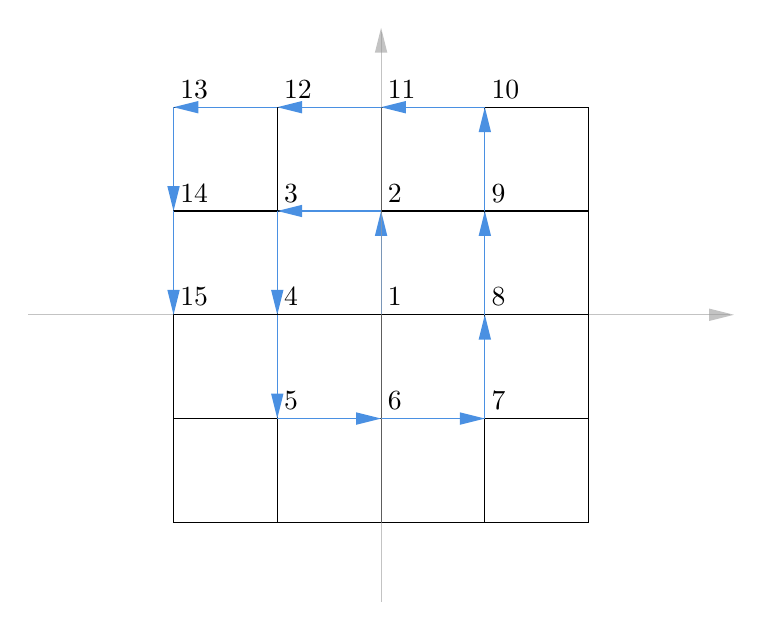
\begin{tikzpicture}[x=0.75pt,y=0.75pt,yscale=-1,xscale=1]
%uncomment if require: \path (0,320); %set diagram left start at 0, and has height of 320

%Straight Lines [id:da8721096924770437] 
\draw [color={rgb, 255:red, 155; green, 155; blue, 155 }  ,draw opacity=0.6 ]   (37.5,160.06) -- (375.5,160.06) ;
\draw [shift={(377.5,160.06)}, rotate = 180] [fill={rgb, 255:red, 155; green, 155; blue, 155 }  ,fill opacity=0.6 ][line width=0.08]  [draw opacity=0] (12,-3) -- (0,0) -- (12,3) -- cycle    ;
%Shape: Square [id:dp3534096151932711] 
\draw   (107.5,60.06) -- (157.5,60.06) -- (157.5,110.06) -- (107.5,110.06) -- cycle ;
%Shape: Square [id:dp962452328883916] 
\draw   (157.5,60.06) -- (207.5,60.06) -- (207.5,110.06) -- (157.5,110.06) -- cycle ;
%Shape: Square [id:dp005646905585411588] 
\draw   (107.5,110.06) -- (157.5,110.06) -- (157.5,160.06) -- (107.5,160.06) -- cycle ;
%Shape: Square [id:dp30082770905964096] 
\draw   (157.5,110.06) -- (207.5,110.06) -- (207.5,160.06) -- (157.5,160.06) -- cycle ;
%Shape: Square [id:dp5127709876793147] 
\draw   (207.5,60.06) -- (257.5,60.06) -- (257.5,110.06) -- (207.5,110.06) -- cycle ;
%Shape: Square [id:dp10041163486865123] 
\draw   (207.5,110.06) -- (257.5,110.06) -- (257.5,160.06) -- (207.5,160.06) -- cycle ;
%Shape: Square [id:dp09251279261434542] 
\draw   (107.5,160.06) -- (157.5,160.06) -- (157.5,210.06) -- (107.5,210.06) -- cycle ;
%Shape: Square [id:dp8494572450517244] 
\draw   (157.5,160.06) -- (207.5,160.06) -- (207.5,210.06) -- (157.5,210.06) -- cycle ;
%Shape: Square [id:dp6861043430326614] 
\draw   (207.5,160.06) -- (257.5,160.06) -- (257.5,210.06) -- (207.5,210.06) -- cycle ;
%Straight Lines [id:da6255734967837832] 
\draw    (157.5,60.06) -- (157.5,110.06) ;
%Straight Lines [id:da699812619321065] 
\draw [color={rgb, 255:red, 74; green, 144; blue, 226 }  ,draw opacity=1 ]   (157.5,110.06) -- (157.5,158.06) ;
\draw [shift={(157.5,160.06)}, rotate = 270] [fill={rgb, 255:red, 74; green, 144; blue, 226 }  ,fill opacity=1 ][line width=0.08]  [draw opacity=0] (12,-3) -- (0,0) -- (12,3) -- cycle    ;
%Straight Lines [id:da11271119855851008] 
\draw    (107.5,110.06) -- (157.5,110.06) ;
%Straight Lines [id:da08372172460589344] 
\draw    (207.5,60.06) -- (207.5,110.06) ;
%Straight Lines [id:da7400912888169191] 
\draw    (157.5,160.06) -- (207.5,160.06) ;
%Straight Lines [id:da1472049419375816] 
\draw    (107.5,160.06) -- (157.5,160.06) ;
%Straight Lines [id:da06264144592693555] 
\draw [color={rgb, 255:red, 74; green, 144; blue, 226 }  ,draw opacity=1 ]   (157.5,160.06) -- (157.5,208.06) ;
\draw [shift={(157.5,210.06)}, rotate = 270] [fill={rgb, 255:red, 74; green, 144; blue, 226 }  ,fill opacity=1 ][line width=0.08]  [draw opacity=0] (12,-3) -- (0,0) -- (12,3) -- cycle    ;
%Straight Lines [id:da8227019785980083] 
\draw [color={rgb, 255:red, 74; green, 144; blue, 226 }  ,draw opacity=1 ]   (207.5,112.06) -- (207.5,160.06) ;
\draw [shift={(207.5,110.06)}, rotate = 90] [fill={rgb, 255:red, 74; green, 144; blue, 226 }  ,fill opacity=1 ][line width=0.08]  [draw opacity=0] (12,-3) -- (0,0) -- (12,3) -- cycle    ;
%Straight Lines [id:da6036919265566432] 
\draw    (207.5,160.06) -- (207.5,210.06) ;
%Straight Lines [id:da7566856786744875] 
\draw    (207.5,110.06) -- (257.5,110.06) ;
%Straight Lines [id:da5752076844169731] 
\draw    (207.5,160.06) -- (257.5,160.06) ;
%Straight Lines [id:da6696997850807531] 
\draw [color={rgb, 255:red, 74; green, 144; blue, 226 }  ,draw opacity=1 ]   (159.5,110.06) -- (207.5,110.06) ;
\draw [shift={(157.5,110.06)}, rotate = 0] [fill={rgb, 255:red, 74; green, 144; blue, 226 }  ,fill opacity=1 ][line width=0.08]  [draw opacity=0] (12,-3) -- (0,0) -- (12,3) -- cycle    ;
%Straight Lines [id:da5283919090418059] 
\draw    (257.5,60.06) -- (257.5,110.06) ;
%Shape: Square [id:dp12621580840019253] 
\draw   (257.5,110.06) -- (307.5,110.06) -- (307.5,160.06) -- (257.5,160.06) -- cycle ;
%Shape: Square [id:dp2378676663787076] 
\draw   (257.5,160.06) -- (307.5,160.06) -- (307.5,210.06) -- (257.5,210.06) -- cycle ;
%Shape: Square [id:dp535339782784388] 
\draw   (257.5,60.06) -- (307.5,60.06) -- (307.5,110.06) -- (257.5,110.06) -- cycle ;
%Shape: Square [id:dp08438308557851948] 
\draw   (107.5,210.06) -- (157.5,210.06) -- (157.5,260.06) -- (107.5,260.06) -- cycle ;
%Shape: Square [id:dp20253737983709263] 
\draw   (157.5,210.06) -- (207.5,210.06) -- (207.5,260.06) -- (157.5,260.06) -- cycle ;
%Shape: Square [id:dp46829799638578296] 
\draw   (207.5,210.06) -- (257.5,210.06) -- (257.5,260.06) -- (207.5,260.06) -- cycle ;
%Shape: Square [id:dp4461549772168607] 
\draw   (257.5,210.06) -- (307.5,210.06) -- (307.5,260.06) -- (257.5,260.06) -- cycle ;
%Straight Lines [id:da4915028841257445] 
\draw [color={rgb, 255:red, 74; green, 144; blue, 226 }  ,draw opacity=1 ]   (257.5,162.06) -- (257.5,210.06) ;
\draw [shift={(257.5,160.06)}, rotate = 90] [fill={rgb, 255:red, 74; green, 144; blue, 226 }  ,fill opacity=1 ][line width=0.08]  [draw opacity=0] (12,-3) -- (0,0) -- (12,3) -- cycle    ;
%Straight Lines [id:da8079303021987698] 
\draw    (257.5,210.06) -- (257.5,260.06) ;
%Straight Lines [id:da6637957221418753] 
\draw    (207.5,210.06) -- (207.5,260.06) ;
%Straight Lines [id:da3540823746572441] 
\draw    (157.5,210.06) -- (157.5,260.06) ;
%Straight Lines [id:da8685001030610524] 
\draw    (157.5,210.06) -- (157.5,260.06) ;
%Straight Lines [id:da13528159745797708] 
\draw    (107.5,210.06) -- (157.5,210.06) ;
%Straight Lines [id:da891955148720676] 
\draw    (257.5,110.06) -- (307.5,110.06) ;
%Straight Lines [id:da5743341846119796] 
\draw    (257.5,160.06) -- (307.5,160.06) ;
%Straight Lines [id:da08665804634756435] 
\draw    (257.5,210.06) -- (307.5,210.06) ;
%Straight Lines [id:da36299958438292634] 
\draw [color={rgb, 255:red, 74; green, 144; blue, 226 }  ,draw opacity=1 ]   (157.5,210.06) -- (205.5,210.06) ;
\draw [shift={(207.5,210.06)}, rotate = 180] [fill={rgb, 255:red, 74; green, 144; blue, 226 }  ,fill opacity=1 ][line width=0.08]  [draw opacity=0] (12,-3) -- (0,0) -- (12,3) -- cycle    ;
%Straight Lines [id:da9649089451630455] 
\draw [color={rgb, 255:red, 74; green, 144; blue, 226 }  ,draw opacity=1 ]   (207.5,210.06) -- (255.5,210.06) ;
\draw [shift={(257.5,210.06)}, rotate = 180] [fill={rgb, 255:red, 74; green, 144; blue, 226 }  ,fill opacity=1 ][line width=0.08]  [draw opacity=0] (12,-3) -- (0,0) -- (12,3) -- cycle    ;
%Straight Lines [id:da29495643346675915] 
\draw [color={rgb, 255:red, 155; green, 155; blue, 155 }  ,draw opacity=0.6 ]   (207.5,298.34) -- (207.5,23.79) ;
\draw [shift={(207.5,21.79)}, rotate = 90] [fill={rgb, 255:red, 155; green, 155; blue, 155 }  ,fill opacity=0.6 ][line width=0.08]  [draw opacity=0] (12,-3) -- (0,0) -- (12,3) -- cycle    ;
%Straight Lines [id:da8999856233681163] 
\draw [color={rgb, 255:red, 74; green, 144; blue, 226 }  ,draw opacity=1 ]   (257.5,62.06) -- (257.5,110.06) ;
\draw [shift={(257.5,60.06)}, rotate = 90] [fill={rgb, 255:red, 74; green, 144; blue, 226 }  ,fill opacity=1 ][line width=0.08]  [draw opacity=0] (12,-3) -- (0,0) -- (12,3) -- cycle    ;
%Straight Lines [id:da5890444457373256] 
\draw [color={rgb, 255:red, 74; green, 144; blue, 226 }  ,draw opacity=1 ]   (257.5,112.06) -- (257.5,160.06) ;
\draw [shift={(257.5,110.06)}, rotate = 90] [fill={rgb, 255:red, 74; green, 144; blue, 226 }  ,fill opacity=1 ][line width=0.08]  [draw opacity=0] (12,-3) -- (0,0) -- (12,3) -- cycle    ;
%Straight Lines [id:da337322378639602] 
\draw [color={rgb, 255:red, 74; green, 144; blue, 226 }  ,draw opacity=1 ]   (209.5,60.06) -- (257.5,60.06) ;
\draw [shift={(207.5,60.06)}, rotate = 0] [fill={rgb, 255:red, 74; green, 144; blue, 226 }  ,fill opacity=1 ][line width=0.08]  [draw opacity=0] (12,-3) -- (0,0) -- (12,3) -- cycle    ;
%Straight Lines [id:da2568587995669316] 
\draw [color={rgb, 255:red, 74; green, 144; blue, 226 }  ,draw opacity=1 ]   (159.5,60.06) -- (207.5,60.06) ;
\draw [shift={(157.5,60.06)}, rotate = 0] [fill={rgb, 255:red, 74; green, 144; blue, 226 }  ,fill opacity=1 ][line width=0.08]  [draw opacity=0] (12,-3) -- (0,0) -- (12,3) -- cycle    ;
%Straight Lines [id:da5289313288344057] 
\draw [color={rgb, 255:red, 74; green, 144; blue, 226 }  ,draw opacity=1 ]   (109.5,60.06) -- (157.5,60.06) ;
\draw [shift={(107.5,60.06)}, rotate = 0] [fill={rgb, 255:red, 74; green, 144; blue, 226 }  ,fill opacity=1 ][line width=0.08]  [draw opacity=0] (12,-3) -- (0,0) -- (12,3) -- cycle    ;
%Straight Lines [id:da2835668925548698] 
\draw [color={rgb, 255:red, 74; green, 144; blue, 226 }  ,draw opacity=1 ]   (107.5,108.06) -- (107.5,60.06) ;
\draw [shift={(107.5,110.06)}, rotate = 270] [fill={rgb, 255:red, 74; green, 144; blue, 226 }  ,fill opacity=1 ][line width=0.08]  [draw opacity=0] (12,-3) -- (0,0) -- (12,3) -- cycle    ;
%Straight Lines [id:da8793967428018006] 
\draw [color={rgb, 255:red, 74; green, 144; blue, 226 }  ,draw opacity=1 ]   (107.5,158.06) -- (107.5,110.06) ;
\draw [shift={(107.5,160.06)}, rotate = 270] [fill={rgb, 255:red, 74; green, 144; blue, 226 }  ,fill opacity=1 ][line width=0.08]  [draw opacity=0] (12,-3) -- (0,0) -- (12,3) -- cycle    ;

% Text Node
\draw (209.5,157.06) node [anchor=south west] [inner sep=0.75pt]   [align=left] {1};
% Text Node
\draw (209.5,107.06) node [anchor=south west] [inner sep=0.75pt]   [align=left] {2};
% Text Node
\draw (159.5,107.06) node [anchor=south west] [inner sep=0.75pt]   [align=left] {3};
% Text Node
\draw (159.5,157.06) node [anchor=south west] [inner sep=0.75pt]   [align=left] {4};
% Text Node
\draw (159.5,207.06) node [anchor=south west] [inner sep=0.75pt]   [align=left] {5};
% Text Node
\draw (209.5,207.06) node [anchor=south west] [inner sep=0.75pt]   [align=left] {6};
% Text Node
\draw (259.5,207.06) node [anchor=south west] [inner sep=0.75pt]   [align=left] {7};
% Text Node
\draw (259.5,157.06) node [anchor=south west] [inner sep=0.75pt]   [align=left] {8};
% Text Node
\draw (259.5,107.06) node [anchor=south west] [inner sep=0.75pt]   [align=left] {9};
% Text Node
\draw (259.5,57.06) node [anchor=south west] [inner sep=0.75pt]   [align=left] {10};
% Text Node
\draw (209.5,57.06) node [anchor=south west] [inner sep=0.75pt]   [align=left] {11};
% Text Node
\draw (159.5,57.06) node [anchor=south west] [inner sep=0.75pt]   [align=left] {12};
% Text Node
\draw (109.5,57.06) node [anchor=south west] [inner sep=0.75pt]   [align=left] {13};
% Text Node
\draw (109.5,107.06) node [anchor=south west] [inner sep=0.75pt]   [align=left] {14};
% Text Node
\draw (109.5,157.06) node [anchor=south west] [inner sep=0.75pt]   [align=left] {15};


\end{tikzpicture}

    \caption{二维正方晶格的格点编号方案}
    \label{fig:site-index-2d}
\end{figure}

二维Hubbard模型的数值bootstrap方法大体上和一维Hubbard模型一致。
我们还是以\eqref{eq:operator-space-criteria}为截断算符空间的标准。如何搜索满足这个条件的算符需要一些额外的说明。
在二维情况下,直接暴力枚举满足\eqref{eq:inequality-hubbard-opstr}是非常低效的,因为涉及到的格点数目大体上为$K^2$量级,于是需要遍历$4^{K^2}$量级的湮灭算符乘积。
为了保证构成$H$的算符出现在截断后的算符空间中,至少需要$K=4$,于是需要遍历\num{4e9}个算符,而且随着$K$增大指数增长。
我们使用深度优先搜索来简化计算,在\prettyref{fig:site-index-2d}中按照格点编号从小到大的顺序,依次放置以下四种算符组合之一:没有算符,有一个自旋向上的湮灭算符,有一个自旋向下的湮灭算符,同时有自旋向上和向下的湮灭算符。
一旦发现$l(O) \leq K$条件不满足,立即“剪枝”,并且切换到下一个算符组合。
如此可以大大加速算符空间的搜索速度。

二维Hubbard模型的对称性除了\prettyref{sec:symbolic-hubbard}中提到的对称性以外,还包括$C_4$旋转对称性。
这一对称性可以通过类似于平移对称性的方式,通过将QuantumAlgebra.jl算符上的坐标标签修改为旋转\SI{90}{\degree}后的坐标标签来施加。

\subsection{计算结果}\label{sec:hubbard-2d-result}

% data obtained by running hubbard-2d-prototype\main.jl.

\begin{table}
    \caption{$K = 8$时的二维Hubbard模型的线性SDP结果,参考值取自\parencite{han_manybody}的表2和表3}
    \label{tbl:hubbard-2d-linear-sdp}
    \centering
    \begin{tabular}{cccccc}
        \toprule
        \multicolumn{2}{c}{$n_i=1$}                                 & $U=2$   & $U=4$   & $U=6$   & $U=8$  \\
        \midrule
        \multirow{2}{*}{$K=8$}     & $E$                               & -1.3164 & -1.0491 & -0.8626 & -0.7276  \\
                                    & $n_{i \uparrow} n_{i \downarrow}$ &  0.1602 &  0.1105 &  0.0784 &  0.0576  \\
        \midrule
        \multirow{2}{*}{DMRG参考值}  & $E$                               & -1.176(1) & -0.8605(5) & -0.6565(1) & -0.5241(1)  \\
                                    & $n_{i \uparrow} n_{i \downarrow}$ &  0.188(1) &  0.126(1) &  0.0809(3) &  0.0539(1)  \\
        \bottomrule
    \end{tabular}
\end{table}

显然,二维数值bootstrap涉及比一维更多的算符,从而内存空间是一个主要的计算瓶颈。由于时间关系,本文未能完成较大规模的二维Hubbard模型数值bootstrap计算,目前获得的结果如\prettyref{tbl:hubbard-2d-linear-sdp}。此处获得的下界过于宽松,但双占据相对准确。更精确的二维Hubbard模型的计算有待进一步研究。%
\footnote{
    本节使用的程序的执行入口见\url{https://github.com/wujinq/numerical-boostrap/blob/main/hubbard-2d-prototype/main.jl}。
}%

\chapter{总结与展望}\label{chap:future}

本文回顾了数值bootstrap技术的形式理论,完成了非简谐振子的线性SDP和非线性SDP数值bootstrap,以及一维和二维Hubbard模型的数值bootstrap,并使用其它数值方法做了基准测试,其中非简谐振子的线性SDP、掺杂一维Hubbard模型的线性SDP未见已有文献报道。
数值bootstrap无符号问题,能够给出系统能量严格下界,可以计算算符空间$\mathcal{C}$中的全部算符的期望值,从而原则上可以较为精确地计算任意多点关联函数,根据\eqref{eq:operator-bound}可以和张量网络方法配合获取任意物理量的期望值的上下界,并且完全不依赖哈密顿量中涉及的自由度的类型,这些特征意味着数值bootstrap方法在解决非微扰物理问题上有非常巨大的潜力。

本章将回顾前文中遇到的问题,并讨论未来可能的研究方向。

\section{非简谐振子的线性SDP的收敛性问题}

非简谐振子的线性SDP未见文献报道,一方面可能因为非线性SDP可以非常简洁地解决此问题,一方面可能就是因为收敛性问题。
定位\prettyref{sec:convergence-problem}中提到的收敛性问题的根源,并且检查它是否在其它类型的问题中也有出现是必要的。
可能的因素包括\prettyref{sec:convergence-problem}中提到的浮点数精度不足,以及\prettyref{sec:hubbard-1d-result}中提到的\eqref{eq:complex-to-real}构造引入收敛性问题的可能性。
前一种可能性需要通过调整求解器精度加以验证。就后一种可能性,一种验证方式是,对$x$-$p$自由度的系统同样可以定义(玻色型)产生湮灭算符,非简谐振子的基态波函数是实的,从而在粒子数表象中$\expval*{(a^\dagger)^m a^n}$也是实的,因此我们可以将\prettyref{chap:hubbard}中的方法套用到使用产生湮灭算符的语言表述的非简谐振子上,做一个纯实数,不包含\eqref{eq:complex-to-real}构造的线性SDP的数值bootstrap。
如果这样收敛性良好,那说明\eqref{eq:complex-to-real}构造是不利于收敛性的,在未来的线性SDP计算中应该避免。

\section{算符空间和约束的选取}\label{sec:operator-space-constraint}

从\prettyref{fig:ground-state-e-x2-plot}可以看出,在非简谐振子问题中决定了能量下界的约束实际上只有一个——不同约束导致的可行域边界的连接点是不光滑的,而能量最小值点显然没有取在某个不光滑的点上。
这提示我们,为了获得基态能量,实际上并不需要全部的约束。如果有方法能够判断出在一个问题中,给基态能量下界设下限制的约束条件主要是什么,那么计算效率可以大大提高,因为本文考虑的Hubbard模型的线性SDP的性能瓶颈似乎主要在优化问题\emph{之前}(\prettyref{sec:hubbard-1d-result})。
未来可以在不同的模型中撤去一些约束,观察剩下的约束的数值bootstrap的精度是否有显著下降,从而获知哪些等式约束对数值bootstrap是重要的;类似的,可以人为缩小$M$矩阵的规模,观察数值bootstrap的精度,从而获知哪些算符给出的正定性约束是至关重要的。
一种可能的思路是在使用DMRG或其它张量网络方法做基准测试时,观察哪些约束被张量网络解违反得最为厉害——这些约束更加不容易满足,因此直觉上,可能会对系统能量施加更强的约束。

如何选择算符空间同样是需要注意的。\prettyref{sec:hubbard-1d-result}中的结果暗示Hubbard模型中的算符空间的选取需要适合电子的巡游行为,如果要捕捉到电子的巡游行为,就需要使用更加非局域的算符。
同样,张量网络方法基准测试也可能能够帮助这方面的分析:可以先取一个很大的算符空间,观察哪些算符的张量网络估计值较大,就使用这些算符组建$\mathcal{C}$而后进行数值bootstrap。


\section{扩大计算规模和提高精度}

本文在\prettyref{sec:one-dimensional-hubbard}和\prettyref{sec:hubbard-2d}中的计算均没有达到\parencite{han_manybody}的精度,并且\prettyref{sec:hubbard-2d-result}中提到了二维Hubbard模型的数值bootstrap面临内存瓶颈。
如何克服这些瓶颈,追求更高的计算精度也是非常有必要考虑的问题。

除了\prettyref{sec:operator-space-constraint}中提到的丢弃无用的约束和算符以外,也需要进一步设法加快搜索满足$\mathcal{C}$的条件的算符、计算对易子、构建优化问题的速度。
后两者中,不同算符对应的约束条件彼此不相干,在问题规模大时可以考虑并行。
虽然\prettyref{sec:one-dimensional-hubbard}和\prettyref{sec:hubbard-2d}中线性SDP计算速度已经足够好了,不能排除问题规模进一步扩大时,类似于非简谐振子的收敛性问题出现,或者现有的求解器效率不佳,届时可能需要手动实现为数值bootstrap专门优化的求解器。

\section{将数值bootstrap用在更多模型上}

本文仅仅讨论了非简谐振子和Hubbard模型,即只讨论了量子力学中的坐标和动量以及费米子这两类自由度。
非微扰物理体系还涉及更多可能的自由度:自旋,t-J模型中的无双占据态的费米子,玻色子……原则上,只需要指定每种自由度涉及的算符代数以及哈密顿量,即可自动地完成数值bootstrap。

张量网络方法对待研究的系统的波函数结构有所预设,蒙特卡洛方法预设配分函数中不同构型的权重均有足够大的实部,如何修改波函数拟设或是改动辅助场类型来适合待研究的系统是不透明的。
数值bootstrap中不存在这样的预设,影响计算精度的因素较为透明地体现在算符空间和等式约束的选取上,通过增大算符空间可以系统地提升计算精度,这为研究范围极其广阔的凝聚态强关联系统提供了一种新的手段。
不同格点上的Hubbard模型\cite{Ye_2019,PhysRevB.90.081105}和海森堡模型\cite{anderson1973resonating,kagome,Liu_2022}被预言能够产生不同的新奇物态,如类似于高温超导中的赝能隙、各种类型的自旋液体、解禁闭量子相变等,这些模型原则上都可以使用数值bootstrap研究,和已有的数值方法相互印证。

ITensor库将常见的物理自由度对应的张量网络中的张量指标事先实现好,用户只需要调用接口即可\cite{itensor-indices},未来可能可以开发一个类似的数值bootstrap库,用于简化搜索满足条件的算符,建立算符空间,将$\mathcal{C}$中的算符编号,构建优化问题等重复性操作。

% 后置部分包含参考文献、声明页(自动生成)等
\backmatter

% 打印参考文献列表
\printbibliography

\chapter{致\quad 谢}

我首先要感谢戚扬老师。戚老师的课程和讨论班让我对凝聚态物理产生了很强的兴趣。
我对本文中提到的数值方法——DQMC,DMRG,ITensor库,数值bootstrap本身——的第一次接触都是在和戚老师的讨论中获得的。
感谢我的室友和同学:舒畅,王逸舟,赵星祺,郭家祺,王思源,于鑫阳,邵一陆,很幸运大学四年能够认识如此有趣的诸位。
感谢\LaTeX 大师曾祥东学长,感谢他的毕业论文模板——没有这份模板,本文的排版将会非常令人头疼。
感谢我的父母,一句“不要有后顾之忧”,是我在物理道路上继续前进的最大底气。

%\chapter{附\quad 录}

\end{document}
